\chapter[Optimization of the current extracted from an UCIS]{Optimization of the current extracted from an ultracold ion source\label{ch:currentmea}}
%%\documentclass[]{iopart}
%
%%\documentclass[aip,jap,onecolumn,preprint,showpacs]{revtex4}
%%\documentclass[aip,jap,reprint,twocolumn,showpacs,floatfix]{revtex4-1}
%
%\usepackage{graphicx}% Include figure files
%\usepackage{dcolumn}% Align table columns on decimal point1
%\usepackage{bm}% bold math
%\usepackage[caption=false]{subfig}
%%\usepackage[separate-uncertainty = true]{siunitx}
%
%\begin{document}
%
%\title{Optimization of the current extracted from an ultracold ion source}
%
%\author{N Debernardi, R W L van Vliembergen, W J Engelen, K H M Hermans, M P Reijnders, S B van der Geer, P H A Mutsaers, O J Luiten and E J D Vredenbregt}
%\address{Department of Applied Physics, Eindhoven University of Technology, P.O. Box 513, 5600 MB Eindhoven, the Netherlands}
%\ead{E.J.D.Vredenbregt@tue.nl}
%
%\date{\today{}}

\begin{abstract}
Photoionization of trapped atoms is used to create ion beams with milliKelvin transverse temperature. The temporal behavior of the current  that can be extracted from such an ultracold ion source, is measured when operating in a pulsed mode. A number of experimental parameters is varied to find the conditions under which the time-averaged current is maximized. A dynamic model of the source is developed that agrees quite well with the experimental observations. The radiation pressure exerted by the excitation laser beam is found to substantially increase the extracted current. For a source volume with typical root-mean-square radius of 20~$\mu$m, a maximum peak current of 88~pA is observed, limited by the available ionization laser power of 46~mW. The optimum time-averaged current is 13~pA at a 36\% duty cycle. Based on the model, an average current in the 100~pA range is possible at higher ionization laser power. Particle-tracking simulations show that stochastic heating strongly reduces the brightness of the ion beam at higher current for experimental conditions.
\footnote{The work described in this chapter (appendix excluded) by \underline{N. Debernardi}, R.W.L. van Vliembergen, W.J. Engelen, K.H.M. Hermans, M.P. Reijnders, S.B. van der Geer, P.H.A. Mutsaers, O.J. Luiten and E.J.D. Vredenbregt has been submitted for publication to New J. Phys.}
\end{abstract}

%\pacs{32.80.Fb, 41.75.Ak, 37.10.Vz}

%\submitto{\NJP}

%\maketitle
\clearpage

\section{Introduction}
Focused Ion Beam (FIB) instruments are widely used in the semiconductor industry and nanoscience, e.g. for milling and deposition purposes. The FIB is made of two interdependent components: an ion source and a focusing column. Both may have to be improved in order to satisfy the industry's demand of reduction in feature size \cite{itrs,Moore_E_65}. Commercial FIBs use the Liquid-Metal Ion Source (LMIS) because of its high brightness ($10^6$~A/m$^2$~sr~eV) \cite{Hagen_J_08}. A disadvantage of the LMIS is its intrinsic energy spread of 4.5~eV \cite{Bell_JVSTB_88} which is the result of Coulombic interactions due to the high current density near the tip of the source \cite{Hagen_J_08}. This limits the probe size for a fixed current through chromatic aberration \cite{Volkert2007, Kruit_NIaMiPRSAASDaAE_95}. 

An alternative ion source has been proposed for FIBs that is known either as the Magneto-Optical Trap Ion Source (MOTIS) \cite{Hanssen_PRA_06} or as the the Ultra-Cold Ion Source (UCIS) \cite{Geer_JoAP_07}. MOTIS and UCIS are in principle interchangeable source concepts. Both are based on near-threshold photo-ionization of a cloud of laser-cooled and trapped atoms \cite{Metcalf_Book_99}. The essential difference between this type of source and the LMIS is that the current density at the source is much reduced because the current is extracted from an extended area. This potentially reduces Coulombic interactions so that lower energy spread may be achieved. High brightness should then result from a small divergence due to the extremely low temperature of the ions. The source is versatile in the sense that it can be operated with a variety of atomic species \cite{Steele_JVSTB_10} and produces isotopically pure ion beams.

By now it has been established that UCIS/MOTIS can indeed produce ion beams with energy spread far below that of the LMIS (with 20 meV rms energy spread demonstrated \cite{Reijnders_PRL_09}), that the transverse temperature of the ions is close to that of the atoms (with 120$\pm$50~$\mu$K demonstrated for a chromium MOTIS \cite{Hanssen_NL_08}, and 3$\pm$2~mK for a rubidium UCIS \cite{Debernardi_JAP_11}), that ion currents of several tens of pA can be extracted (30~pA demonstrated for a lithium MOTIS \cite{Steele_JAP_11}), and that focusing to sub-micron probe size is possible (200~nm demonstrated with a chromium MOTIS \cite{Steele_JVSTB_10}). In addition, new ways to adjust longitudinal and transverse properties of the extracted ion beams by employing pulsed acceleration fields have been demonstrated \cite{Debernardi_JAP_11,Reijnders_PRL_10,Reijnders_JAP_11}. However, so far the reduced brightness achieved with MOTIS/UCIS ($\approx 10^4$~A/m$^2$~sr~eV, demonstrated for a chromium MOTIS \cite{Hanssen_NL_08}) is substantially lower than the established brightness of a gallium LMIS \cite{Hagen_J_08}, limiting application of the source in FIBs. It is therefore of interest to assess how the brightness of this new type of ion source can be optimized while retaining the essential advantage of low energy spread. 

Maximum brightness and minimum energy spread are in practice achieved under different conditions. In either case, two-step ionization is employed with an excitation laser that first excites the trapped atoms from their ground state to an intermediate excited state, and an ionization laser that takes the excited atoms to just above the ionization threshold. When the entire atom cloud is excited and the ionization beam is directed parallel to the direction of the ion beam \cite{Steele_JAP_11}, the current density is maximized, and, in addition, a continuous ion beam is generated. The disadvantage is that the energy spread of the resulting ion beam is also maximized, because this is proportional to the product of the length of the ionization volume and the ambient electric acceleration field \cite{Reijnders_PRL_09}. Achieving low energy spread then requires a low extraction field, which unfortunately leads to a reduction of the beam brightness due to Coulombic interactions \cite{Geer_JoAP_07,Steele_JAP_11}. If, on the other hand, only a small volume of the entire cloud of atoms is selected by crossing the excitation laser beam with the ionization laser beam at the center of the atomic cloud \cite{Geer_JoAP_07,Debernardi_JAP_11,Reijnders_PRL_10,Reijnders_JAP_11}, a proportionally lower energy spread at the same extraction field can be achieved. However, because the ionization volume is smaller, less current is extracted, and, in addition, pulsed operation of the source is required. 

In this paper we show that it is possible in principle to obtain both minimum energy spread (same experimental conditions as in \cite{Reijnders_PRL_09}) and maximum extracted current. We find that the current extracted from a small source volume can be substantially larger than previously predicted \cite{Geer_JoAP_07} due to the radiation pressure that the excitation laser beam exerts. This causes atoms initially outside the selected ionization volume to contribute to the ion current, enhancing the brightness of the source. We first give a detailed description of the UCIS in section \ref{seq:setup}. Then we predict the conditions under which the current extracted from the source should be optimized in section \ref{sec:model}. We report on experiments to establish the parameters of the model in subsection \ref{sec:param} and to validate the model in Subsection \ref{sec:verify}. Finally, we use the source model to predict what may finally be achieved in section \ref{sec:conclusion}, and also consider the influence of stochastic heating on source brightness. We conclude that, due to this stochastic heating, the UCIS in its present form can not yet provide a brightness compatible with the LMIS, even under the optimized conditions developed here.

\section{Experimental setup}
\label{seq:setup}
The UCIS is based on the technique of laser cooling and trapping of neutral atoms \cite{Metcalf_Book_99, Foot_Book_05}. We start with a magneto-optical trap of rubidium atoms: three orthogonal pairs of counter propagating 780 nm laser beams (trapping laser beams) are used to Doppler cool a $^{85}$Rb atomic cloud and a quadrupole magnetic field is added to trap the atoms. Each trapping laser beam has a radius of $\approx$~15 mm and an intensity of $\approx$~100 W$/$m$^2$. Typically $10^8$ Rb-atoms are trapped in a \textit{rms}-radius $\sigma_M=0.8$ mm at an expected source temperature as low as the Doppler temperature $T_D= 143$ $\mu$K \cite{Metcalf_Book_99}. 

The center of the MOT is at the origin of the reference system. The MOT is surrounded by an accelerator \cite{Taban_PRSAB_08}. The accelerator has a cylindrically symmetric structure and it is placed in a vacuum chamber where the pressure is about $10^{-8}$~mbar. Figure \ref{fig:setup} shows a schematic drawing of the experimental setup. The electric field strength at the starting point $z_0$ is 0.37 kV/cm per kV input voltage $V_a$ and the kinetic energy of the extracted ions is $U=e V_a/2.05$, where $e$ is the elementary charge. An ion gains about half of energy applied to the electrodes since the MOT is located half way in between the two electrodes \cite{Taban_PRSAB_08}. An acceleration voltage $V_a=800$~V is used for the experiments described in this paper.
\begin{figure}[tbh!]
    \centering
        \includegraphics[width=0.7\linewidth]{pics/currmea/setup.eps}
    \caption{Schematic view of the experimental setup (not to scale) in the x-z plane. The ionization laser beam and the excitation laser beam select a portion of the Rb atomic cloud trapped inside the accelerator. The ions are accelerated in a DC electric field and after a flight distance of 1.5 m they reach a MCP detector with a phosphor screen. An oscilloscope is connected to the phosphor screen, via a trans-impedance amplifier, to acquire the produced signal.}
    \label{fig:setup}
\end{figure}
For details of the accelerator structure and the experimental setup see references \cite{Taban_PRSAB_08, Debernardi_JAP_11}.

The core region is the area where the ionization process takes place, which is defined by the overlap of two laser beams. The density of the MOT follows a Gaussian distribution with its maximum in the core region. The ionization mechanism is a 2-step process: an excitation laser beam (with wavelength $\lambda_e \approx 780$ nm) excites Rb atoms on the 5s$\rightarrow$5p transition and an ionization laser beam ($\lambda_i = 479.5$ nm) then photo-ionizes the excited 5p atoms with an average maximum power $P_i=$ (46 $\pm$ 4) mW. The trapping laser beams are turned off during the ionization. The size of the core can be changed by varying the size of the laser beams, which are imaged onto two separate CCD cameras virtually positioned at the center of the MOT. The \textit{rms}-radius of the excitation laser is $(23 \times 20)$ $\mu$m$^2$ (respectively in the $x$ and $y$-direction) and the \textit{rms}-radius of the ionization laser is $(53 \times 31)$ $\mu$m$^2$ (in the $x$ and $z$-direction). This results is a core volume $V_c=(2 \pi)^{3/2}(21 \times 20 \times 31)~\mu$m$^3=2 \times 10^{-13}$ m$^3$ (where the $x$-direction has been composed according to \cite{Debernardi_JAP_11}), which is used for the measurements presented in this paper, except where indicated. The power of the excitation laser beam can be varied with the use of an acousto-optic modulator (AOM). The saturation parameter of the laser is given by
\begin{equation}
	s_0 = 0.4 \cdot \frac{I_e}{I_s},
  \label{eq:s0}
\end{equation}
where $I_e$ is the excitation laser beam intensity and $I_s=16.4$ W m$^{-2}$ is the saturation intensity for the rubidium transition of interest. The factor 0.4 is an effective relative transition strength. 
The power of the ionization laser beam can be varied by placing a neutral density filter in the beam's path. 

A double multichannel plate (MCP) detector with phosphor screen is located at 1.5 m from the center of the MOT at $z=0$. The temporal distribution of the current signal is recorded on a oscilloscope by using a trans-impedance amplifier connected to a phosphor screen. The combination of amplifier and MCP has been calibrated (resulting in 6~\% uncertainty) for Rb-85 ion bunches of 390 eV energy (corresponding to $V_a=800$ V). A grounded metal grid in front of the detector (spacing of 5 $\mu$m, 50~\% open fraction) is used to shield the electric field of the MCP.

A programmable pulse generator (PPG) module controls the timing of the experiments with a resolution of 10 ns. Both the extraction of the ions and the acquisition of the data have been automated with the use of several computer programs.

\section{Source model}
\label{sec:model}
A model that describes the operation of the source is needed in order to predict the behavior of the extracted current. The source operates in a quasi-continuous mode, with high repetition rates (it is possible up to 100 kHz, but in the following discussion we work with a frequency of at most a few kHz), alternating a loading phase with a duration $t_l$, in which new atoms are loaded in the trap and an ionization phase with duration $t_i$, when an ion current pulse is extracted from the source. Two relaxation phases with a duration of 5 $\mu$s are alternated in between. The relaxation phases are short compared to the loading and ionization phases. The total period of the sequence is given by $t_{cycle} = t_l + t_e$, where $t_e = t_i + 10~\mu$s is the expansion time, during which the trapping lasers are turned off.

The trapped atom cloud can be divided into two parts, schematically represented in figure~\ref{fig:source}. The inner part, or \emph{core}, contains $N_c$ atoms in an \textit{rms}-radius $\sigma_c$ and the outer part, or \emph{reservoir}, contains $N$ atoms in an \textit{rms}-radius $\sigma_M$ ($\sigma_M \gg \sigma_c$).
\begin{figure}[tbh!]
    \centering
        \includegraphics[width=0.5\linewidth]{pics/currmea/source3.eps}
    \caption{Schematic representation of the source, not to scale. The source is a MOT with a loading rate of new atoms $R_L$. The source is divided in two regions by a surface $\Sigma$: the inner one is the core region with $N_c$ atoms in an \textit{rms}-radius $\sigma_c$, and the outer one is the reservoir region with $N$ atoms in an \textit{rms}-radius $\sigma_M$. The core region is defined by the overlap of the excitation and the ionization laser beams. A pulsed current $I(t)$ of ions is extracted from the core region.}
    \label{fig:source}
\end{figure}
The reservoir and the core are separated by a surface $\Sigma$. The volume of the core $V_c$ is negligible compared to the volume of the reservoir $V_r$, which is approximated to be the volume of the whole MOT ($V_M \approx V_r$). The density in the core $n_c$ is assumed to be uniform due to the small dimension of its radius compared to the radius of the MOT.\\

\subsection{Number of atoms} During the loading phase, atoms from the background vapor are loaded into the MOT at a constant loading rate $R_L$ \cite{Monroe_PRL_90}. Atoms are lost from the trap primarily because of collisions of trapped atoms with the background gas. The loading of the MOT is described by the rate equation
\begin{equation}
	\frac{d N}{d t} = R_L- \frac{N}{\tau_M} ,
  \label{eq:RL_rate}
\end{equation}
with the number of trapped atoms $N$ and the lifetime of the MOT $\tau_M$. In contrast, during the expansion phase $R_L=0$ and the atoms can also more easily escape; the lifetime of the MOT during this phase $\tau_M'$ is shorter than $\tau_M$. A set of two differential equations, one for the loading phase and one for the expansion phase, with $N(0) = N(t_{cycle})$ as the periodic boundary condition allows a unique solution for the steady state. %In this case, the lifetimes of the MOT are chosen to be $\tau_M=200$ ms and $\tau'_M=100$ ms, values which are realistic for the setup. 
The sequence's timings, $t_l=1000$ $\mu$s and $t_e=800$ $\mu$s, are typically the highest used in the experiments, and even then, the number of atoms changes only less than 1\% during the sequence (using typical parameter values shown \ref{tab:TypicalValues}). The average number $\langle N \rangle$ of atoms is therefore a good approximation for the number of atoms in the MOT and it can be expressed as
\begin{equation}
	\langle N \rangle = \frac{N_{\infty}}{1 + \zeta~t_e/t_l} \approx N(t),
  \label{eq:aveN}
\end{equation}
with $\zeta = \tau_M / \tau'_M$ and $N_{\infty} = R_L \tau_M$ as the number of atoms when the MOT is loaded ($t \gg \tau_M$). From equation (\ref{eq:aveN}), it follows that if $t_i \rightarrow 0$ (only the loading phase is present), then $\langle N \rangle \approx N_{\infty}$.
Finally, the core atomic density is given by
\begin{equation}
	n_c = \frac{\langle N \rangle}{(2 \pi)^{3/2} \sigma_M^3}.
  \label{eq:density}
\end{equation}

Typical values for the parameters of the model can be found in table \ref{tab:TypicalValues}. These values are used for the figures and calculations found in this section.
\begin{table*}[ht]
	\caption{\label{tab:TypicalValues} Typical values of the parameters used in the model.}
	\begin{center}
		\begin{tabular}{ | l | l | l |}
			\hline
			Parameter & Symbol & Value \\ \hline
			Loading rate & $R_L$ & $2 \times 10^{9}$ atoms/s \\ 
			Increase in velocity time constant & $\tau_v$ & 39 $\mu$s \\
			Lifetime of the MOT (trapping lasers on)& $\tau_M$ & 0.2 s \\ 
			Lifetime of the MOT (trapping lasers off) & $\tau'_M$ & 0.1 s \\
			Average number of particles in the MOT & $\langle N \rangle$ & $2 \times 10^8$ atoms \\
			Core atomic density of the MOT & $n_c$ & $2.5 \times 10^{16}$ m$^{-3}$\\
			\textit{rms}-radius of the MOT & $\sigma_M$ & 0.8 mm \\
			\textit{rms}-radius of the excitation laser beam & $\sigma_e$ & 30 $\mu$m \\
			\textit{rms}-radius of the ionization laser beam & $\sigma_i$ & 40 $\mu$m \\
			Excitation laser wavelength & $\lambda_e$ & 780 nm \\ 
			Ionization laser wavelength & $\lambda_i$ & 479.5 nm \\ 
			Saturation parameter of the excitation laser beam & $s_0$ & 1 \\
			Power of the ionization laser beam & $P_i$ & 50 mW \\
			Ionization cross section & $\sigma_{PI}$ & $1.48 \times 10^{-21}$ m$^2$ \cite{Gabbanini_OC_97}\\
			Ionization time constant & $\tau_i$ & 60 $\mu$s \\
			Diffusion time constant & $\tau_d$ & 350 $\mu$s \\
			Thermal atomic velocity & $\langle v \rangle$ & 0.3 m/s \\
			Doppler temperature of the trapped Rb-85 atoms & $T_D$ & 143 $\mu$K \\
			Capture velocity & $v_c$ & 4.66 m/s \\
			Linewidth of the $^{85}$Rb transition & $\Gamma$ & $5.98 \cdot 2 \pi$ Mrad/s \\
			Detuning of the excitation laser beam & $\delta$ & 0 \\
			\hline
		\end{tabular}
	\end{center}
\end{table*}
\\

\subsection{Pushing effect} An on-resonance excitation laser beam is used to excite the atoms in the core which will be coincidentally ionized with an ionization laser. The excitation laser beam also accelerates the illuminated atoms in the direction of its propagation \cite{Metcalf_Book_99}, so they can eventually reach the core region and be ionized. This effect is named ``pushing effect'' from now on. The atoms get accelerated with an average radiation pressure force in the $z$-direction $F_z$ given by
\begin{equation}
	F_z(v_z) = \hbar k \frac{\Gamma}{2} \frac{s_0}{1+s_0+(2 \delta(v_z) / \Gamma)^2},
  \label{eq:force}
\end{equation}
where $\hbar$ is Dirac's constant, $\Gamma=5.98 \cdot 2 \pi$ Mrad/s is the linewidth of the atomic transition, $k=2 \pi/\lambda_e$ is the magnitude of the wave vector and $\delta(v_z)=-2 \pi v_z(t) / \lambda_e$ is the Doppler shift of the laser beam. The velocity of the atoms in the $z$-direction $v_z(t)$ can be determined from the Newtonian expression $F_z=m~dv_z/dt$, where $m$ is the atomic mass of rubidium. This leads to
\begin{equation}
	%v_z(t) = \frac{v_c}{2} \sqrt{1 +s_0} \left[ \left( \frac{t+\sqrt{\tau_v^2 +t^2}}{\tau_v} \right)^{1/3} - \left( \frac{t+\sqrt{\tau_v^2 +t^2}}{\tau_v} \right)^{-1/3} \right].
	v_z(t) = \frac{v_c}{2} \sqrt{1 +s_0} \left( \alpha^{1/3} - \alpha^{-1/3} \right),
  \label{eq:velocity}
\end{equation}
where $v_c=4.66$ $m/s$ is the capture velocity and
\begin{equation}
	\alpha = \frac{t+\sqrt{\tau_v^2 +t^2}}{\tau_v}
  \label{eq:alpha}
\end{equation}
in which
\begin{equation}
	\tau_v = \frac{1}{3} \frac{(1 + s_0)^{3/2}}{s_0} \frac{2 m}{\hbar k^2}
  \label{eq:tau_v}
\end{equation}
is the time constant for the increase in velocity. A typical value is $\tau_v=39$ $\mu$s for $s_0=1$. The distance traveled in a certain time $t$ is numerically calculated from equation (\ref{eq:velocity}) as
\begin{equation}
  d(t)=\int_0^t{v_z(t)dt}.
  \label{eq:distance}
\end{equation} 

Due to the pushing effect, ionization is not limited to atoms present in core region at the start of the ionization phase, as we previously assumed \cite{Geer_JoAP_07}. Instead, all the atoms in a cylindrically shaped region as shown in figure~\ref{fig:cylGeo} can be pushed through the ionization region and contribute to the current. Hence, the atoms in the cylindrically shaped region $N_{cyl} = N_p + N_c$ need to be considered to determine the number of atoms in the core region. Here $N_p$ is the number of atoms that will be pushed towards the core region and $N_c$ is the number of atoms present in the core region. The relevant geometry is sketched in figure~\ref{fig:cylGeo}.
\begin{figure}[tbh!]
    \centering
        \includegraphics[width=0.7\linewidth]{pics/currmea/CylinderIonisation.eps}
    \caption{A sketch of the geometrical approximation of the source used in the model. The center of the MOT is at $z=0$ and the core region is represented by the smaller cylinder highlighted in gray on the right hand side, with a size $\sqrt{2 \pi}\sigma_i$. The whole cylinder represents the area crossed by the excitation laser beam, with radius $\sqrt{2} \sigma_e$. The total number of atoms in the cylinder $N_{cyl}$ is the sum of the atoms present in the core $N_c$ and the atoms that will be eventually pushed in the core $N_p$.}
    \label{fig:cylGeo}
\end{figure}
In this figure, the center of the MOT is at $z=0$. The core region is the part of the cylinder highlighted in gray matching $|z| < \sqrt{\frac{\pi}{2}} \sigma_i$; $\sigma_i$ is the \textit{rms}-radius of the ionization laser beam and $\sigma_e$ is the \textit{rms}-radius of the excitation laser beam. The factors $\sqrt2$ and $\sqrt{2 \pi}$ are two normalization constants: the effective radius of the cylinder $\sqrt2 \sigma_e$ is chosen such that the area $A_e=2 \pi \sigma_e^2$ is the same for the actual Gaussian laser beam and in this approximated geometry; the length of the core region $\sqrt{2 \pi} \sigma_i$ is chosen such that the volume of the core $V_c=(2 \pi)^{3/2} \sigma_e^2 \sigma_i$ is the same in both descriptions (assuming $\sigma_e=\sigma_i=\sigma_c$).

\subsection{Atoms initially in cylinder} The number of atoms in the core is given by integrating the local cylinder atomic density $n_{cyl}(z)$ as
\begin{equation}
	N_c = \int_{-\sqrt{\frac{\pi}{2}} \sigma_i}^{\sqrt{\frac{\pi}{2}} \sigma_i}{n_{cyl}(z) A_e dz},
  \label{eq:Ncore}
\end{equation}
Note that the integration over the direction perpendicular to the z-axis has been replaced with multiplying by the area $A_e$. This approximation holds since the size of the excitation laser beam is significantly smaller than the size of the MOT ($\sigma_e \ll \sigma_M$). In reality, $n_{cyl}(z) < n(z)$, because atoms have been pushed out of the volume during the previous ionization phase. However, we approximate $n_{cyl}(z) \approx n(z)$, since it holds in the case of long loading times and short ionization times. We are indeed interested in those times where the maximum of the current is expected to occur. For long ionization times and short loading times the current derived from the model will then be larger than in reality since the approximation does not hold anymore, but this is also a less interesting case for the current optimization. After a time $t$, the entire cylinder has been pushed by the excitation laser beam and all the atoms originally present in the volume have been displaced by a distance $d(t)$. Hence, the atoms present in the core region at a time $t$, have originated from a different part of the MOT. This can be incorporated in the model by replacing the density term $n(z)$ with $n(z-d(t))$.

The atoms initially present inside the cylinder are not confined there. They can diffuse out through its surface and may not reach the core region. The outward diffusion rate of particles is given by
\begin{equation}
	%-\frac{d N_{cyl}}{d t}=\int{\frac{n_{cyl}(z) \langle v \rangle dA_{cyl}}{4}}=\frac{\langle v \rangle}{4} \frac{d A_{cyl}}{d V_{cyl}} N_{cyl},
	-\frac{d N_{cyl}}{d t}=\int{\frac{n_{cyl}(z) \langle v \rangle dA_{cyl}}{4}}=\frac{\langle v \rangle}{4} \frac{\sqrt2}{\sigma_e} N_{cyl},
  \label{eq:Rdiffout}
\end{equation}
where $\langle v \rangle$ is the thermal velocity. This equation can be written in terms of the diffusion time constant $\tau_d$ as
\begin{equation}
	-\frac{d N_{cyl}}{d t}=\frac{N_{cyl}}{\tau_d},
  \label{eq:Rdiffout2}
\end{equation}
where $\tau_d$ is given by
\begin{equation}
	\tau_d=\frac{\sigma_e}{2 \sqrt2 \langle v \rangle}.
  \label{eq:tau_e}
\end{equation}
Using a typical value for the thermal velocity $\langle v \rangle = 0.3$ m/s and for the excitation laser beam size $\sigma_e = 30$ $\mu$m, results in $\tau_d = 350$ $\mu$s (see table \ref{tab:TypicalValues}).

All together, the contribution of the atoms that started out in the cylinder to the number of excited atoms in the core region is given by
\begin{equation}
	N_{core}^{(cyl)}(t) = A_e e^{-\frac{t}{\tau_d}} f(s_0,\delta(v_z)) \int_{-\sqrt{\frac{\pi}{2}} \sigma_i}^{\sqrt{\frac{\pi}{2}} \sigma_i}{n(z-d(t)) dz}.
  \label{eq:Ncorecyl_unsolved}
\end{equation}
In equation (\ref{eq:Ncorecyl_unsolved}), $f$ is the excited state fraction of atoms, which can be expressed as
\begin{equation}
	f(s_0,\delta(v_z)) = \frac{1}{2} \frac{s_0}{1+s_0+(2 \delta(v_z) / \Gamma)^2}.
  \label{eq:fraction}
\end{equation}
Equation (\ref{eq:Ncorecyl_unsolved}) can be further simplified by using the midpoint rule to
\begin{equation}
	N_{core}^{(cyl)}(t) \dot{=} (2 \pi)^{(3/2)} \sigma_e^2 \sigma_i n(-d(t)) e^{-\frac{t}{\tau_d}} f(s_0,\delta(v_z)).
  \label{eq:Ncorecyl}
\end{equation}

Figure \ref{fig:Ncorecyl} plots $N_{core}^{(cyl)}(t)$, normalized with its maximum $N_{init} \equiv N_{core}^{(cyl)}(0)$, versus time for three different values of $s_0$.
\begin{figure}[tbh!]
    \centering
        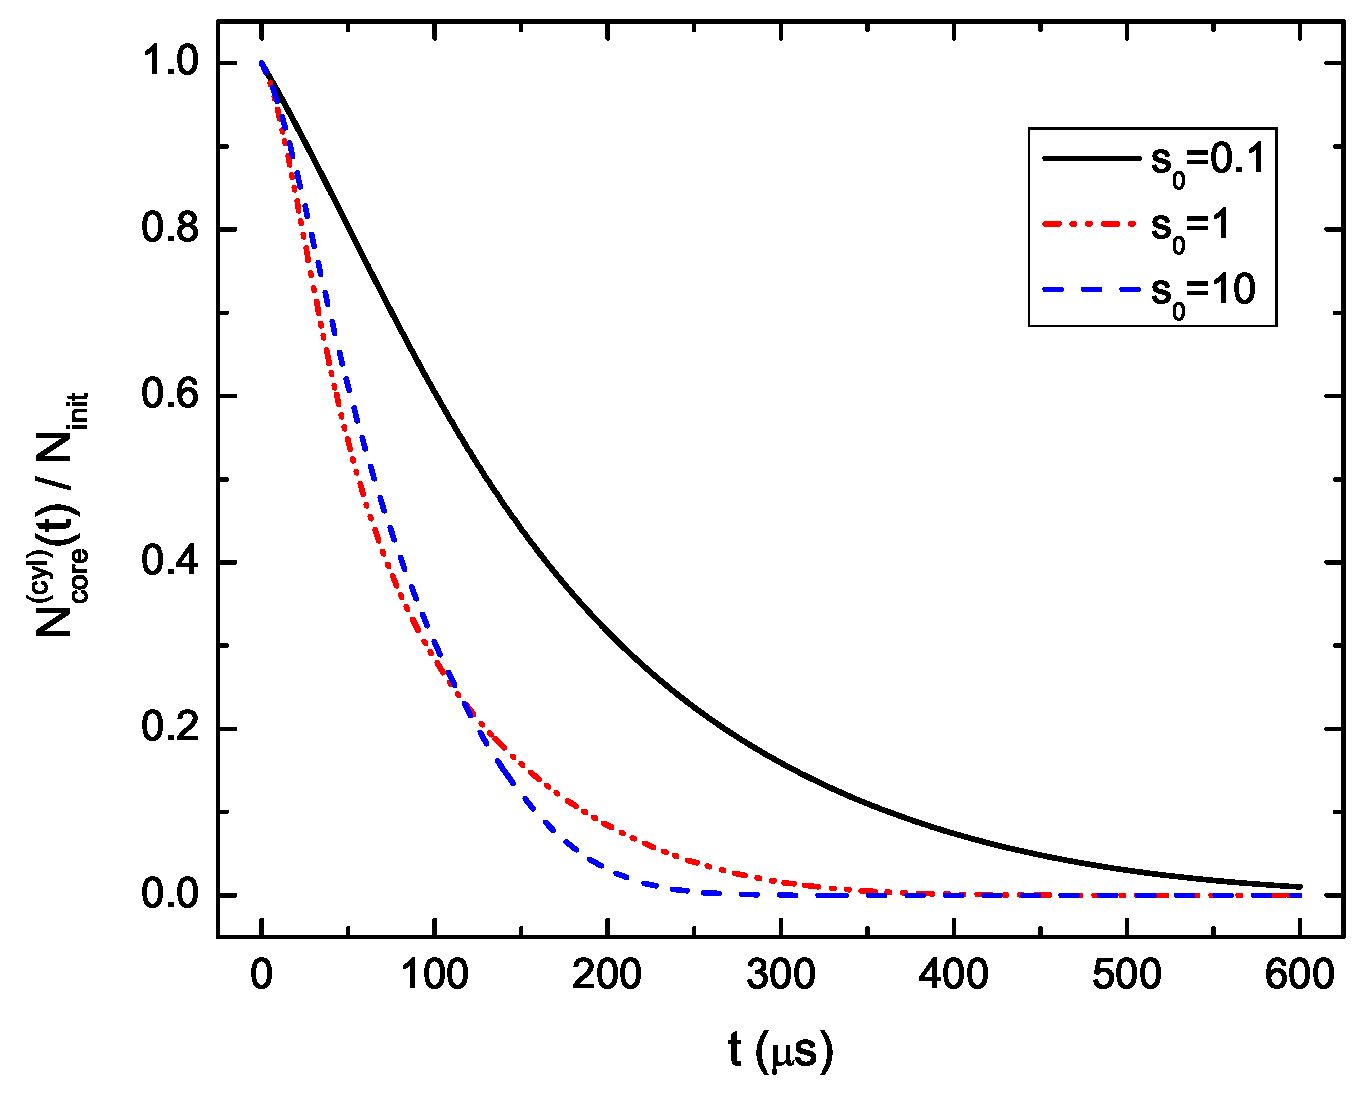
\includegraphics[width=0.7\linewidth]{pics/currmea/Ncyl.eps}
    \caption{A plot of $N_{core}^{(cyl)}(t)$ normalized by its initial value $N_{init}$. Each solid line corresponds to a different $s_0$ parameter of the excitation laser beam. A higher $s_0$ generally means a faster decay in the number of atoms and the pushing effect is more evident. For the smallest $s_0$, the decay is exponential with a time constant $\tau_d$.}
    \label{fig:Ncorecyl}
\end{figure}
This is always a monotonously decreasing function mainly due to the lower density outside the core region. For a very low saturation parameter ($s_0=0.1$) the pushing effect become less important and the dominant loss process of atoms is the diffusion out of the cylinder, which means that the number of atoms decays exponentially with a time constant $\tau_d$.\\

\subsection{Atoms diffusing into the cylinder} 
Apart from the atoms that are present in the cylinder at $t=0$, there is also a contribution of atoms that diffuse into the cylinder. The diffusion flux density into the cylinder is given by
\begin{equation}
	\phi_{diff}^{(in)}(z') = \frac{1}{4} n(z') \langle v \rangle,
  \label{eq:diffin3}
\end{equation}
with $z'$ the coordinate at which a particle enters the cylinder. This flux needs to be integrated over the surface area ($dA_{cyl}=2 \pi \sqrt{2} \sigma_e dz'$) in order to get the inward diffusion flux
\begin{equation}
	\frac{d N_{cyl}}{d t} = \int_{-\infty}^{\sqrt{\frac{\pi}{2}} \sigma_i}{\phi_{diff}^{(in)}(z') 2 \sqrt2 \pi \sigma_e dz'}.
  \label{eq:diffin}
\end{equation}
This rate should be integrated over time to get the number of atoms that have entered the cylinder. However, these atoms can also diffuse out of the cylinder again and only the number of atoms that make it to the core region is interesting for this model.
 
A change of variable $z' = z - d(t')$, where $z$ is the position of a particle which entered the core at a position $z'$ after a time of flight $t'$, is done in order to integrate over the core region instead of over the cylinder,
\begin{equation}
	\frac{d N_{core}^{(diff)}}{d t} = \frac{\pi}{\sqrt2} \sigma_e \langle v \rangle \int_{-\sqrt{\frac{\pi}{2}} \sigma_i}^{\sqrt{\frac{\pi}{2}} \sigma_i} {n(z-d(t)) dz}.
  \label{eq:diffin2}
\end{equation}
Therefore, the contribution of the atoms that diffused into the cylinder to the number of the excited atoms in the core region is given by
\begin{equation}
	N_{core}^{(diff)}(t) \dot{=} \pi^{3/2} \sigma_e \sigma_i \langle v \rangle \int_0^t{n(-d(t')) e^{-\frac{t'}{\tau_d}} f(s_0,\delta) dt'}.
  \label{eq:Ncorediff}
\end{equation}
This expression has also been approximated using the midpoint rule. Note that $N_{core}^{(diff)}(t)$ is the time integral of equation (\ref{eq:Ncorecyl}) apart from some constants.

Figure \ref{fig:Ncorediff} plots $N_{core}^{(diff)}(t)$ for three values of the saturation parameter.
\begin{figure}[tbh!]
    \centering
        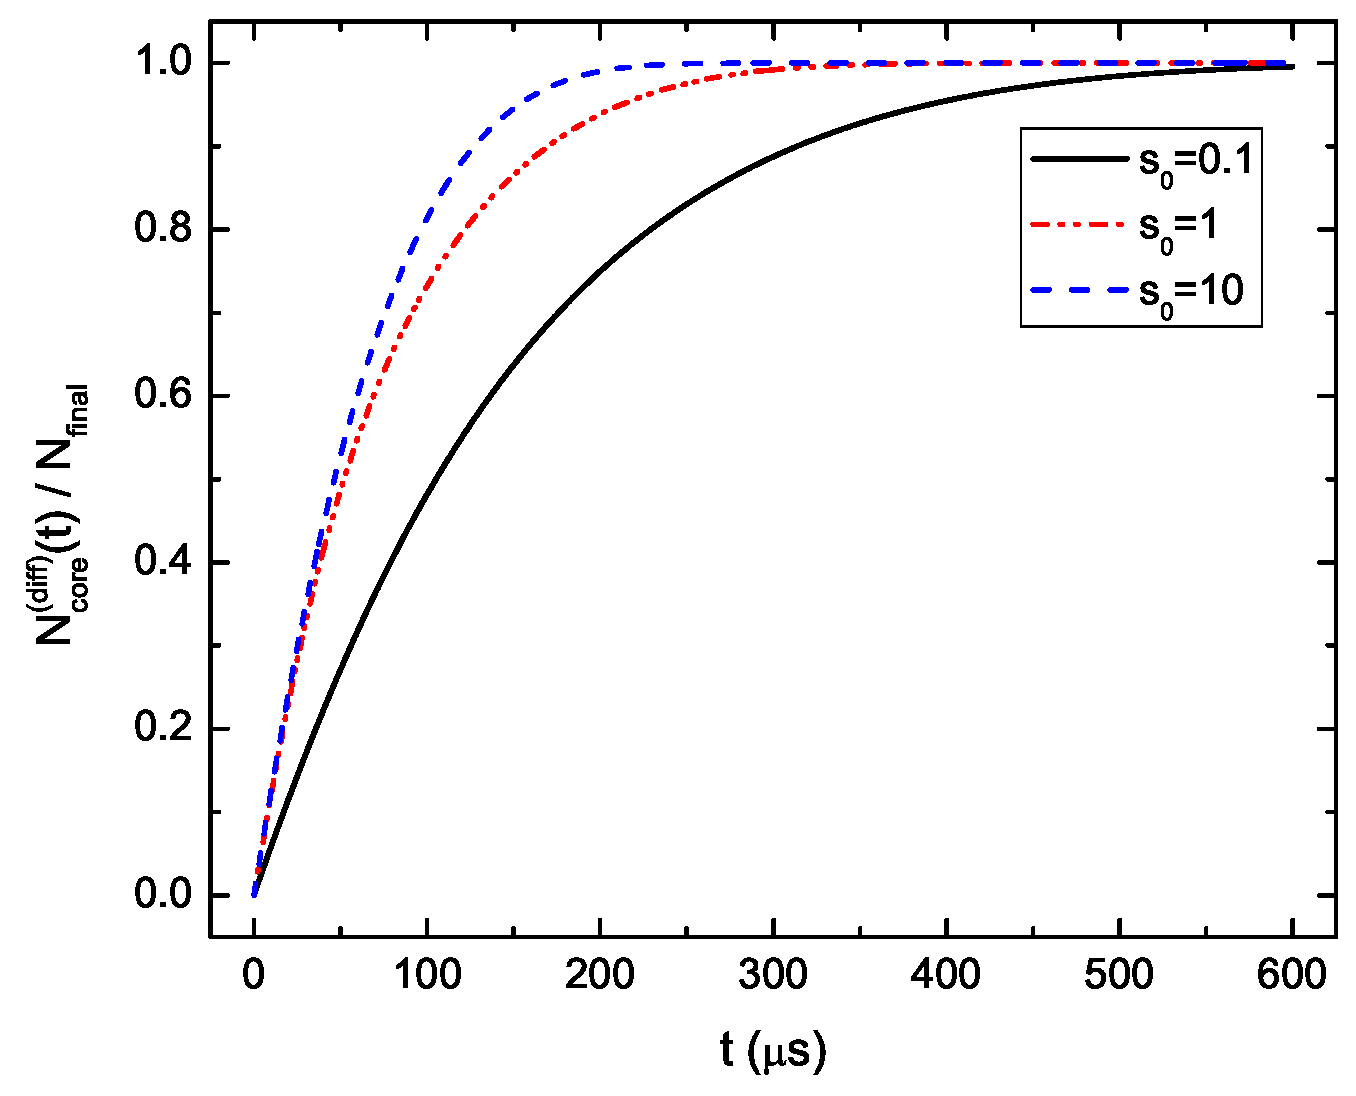
\includegraphics[width=0.7\linewidth]{pics/currmea/Ndiff.eps}
    \caption{A plot of $N_{core}^{(diff)}(t)$ normalized by its initial value $N_{final}$. Each solid line corresponds to a different $s_0$ parameter of the excitation laser beam. A higher $s_0$ generally corresponds to a faster increase in the number of atoms, meaning a stronger ``pushing effect''. For the smallest $s_0$, the increase is exponential with a time constant $\tau_d$.}
    \label{fig:Ncorediff}
\end{figure}
It has been normalized with its maximum value $N_{final} \equiv N_{core}^{(diff)}(\infty)$. This is a monotonously increasing function because at large $t$, the atoms still diffuse into the part of the cylinder close to the core region at the same rate. For a large saturation parameter ($s_0=10$), the convergence to the final value is faster, as for a low saturation parameter the pushing effect is less important.

\subsection{Comparison} Both Figs.\ \ref{fig:Ncorecyl} and \ref{fig:Ncorediff} have been normalized and it is interesting to see how the normalization constants $N_{init}$ and $N_{final}$ relate to each other. This is shown in figure \ref{fig:CompDiffCyl}, where $N_{init}$ and $N_{final}$ are plotted versus $s_0$.
\begin{figure}[tbh!]
    \centering
        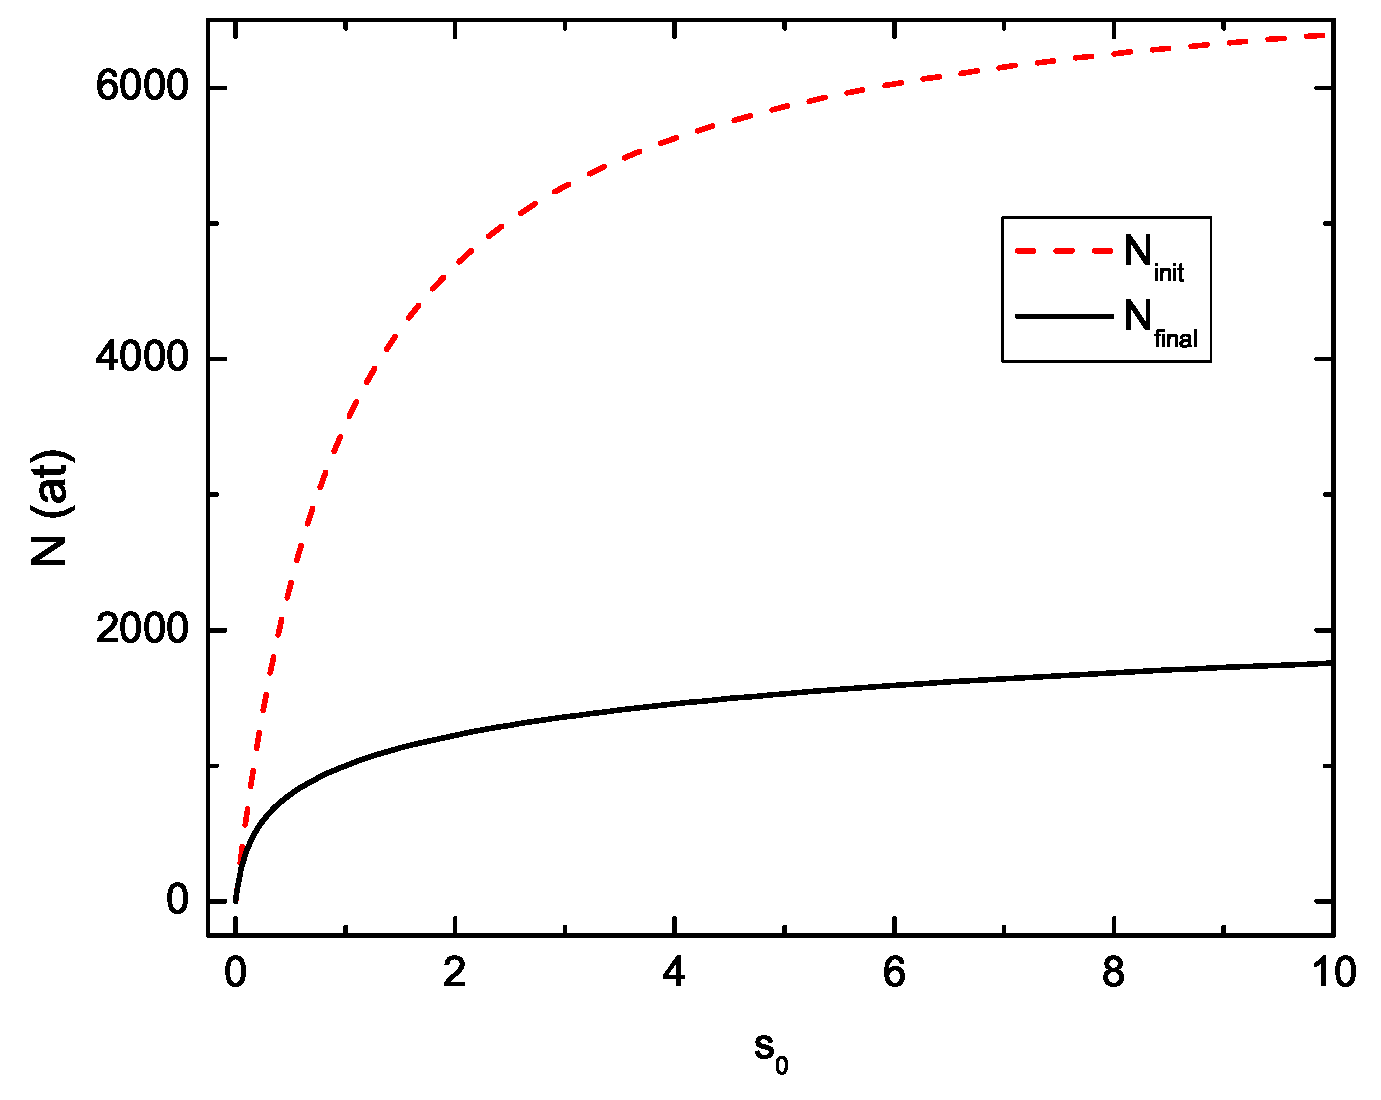
\includegraphics[width=0.7\linewidth]{pics/currmea/Ncyl0AndDiffInf.eps}
    \caption{A plot of $N_{init}$ and $N_{final}$ versus $s_0$. Both are monotonously increasing functions. Hence, a larger saturation parameter is beneficial to the magnitude of both the initial and final currents.}
    \label{fig:CompDiffCyl}
\end{figure}
Both of the functions increase for a larger saturation parameter. Hence, for the current optimization a larger value of the saturation parameter of the excitation laser beam is beneficial. For a finite $s_0$, the following relation holds: $N_{init}>N_{final}$.

\subsection{Extracted current} The ionization rate $r_i$ for excited atoms in the core region can be expressed as
\begin{equation}
    r_i = \tau_i^{-1} = \frac{\sigma_{PI} P_i \lambda_i}{A_i h c},
    \label{eq:r_ion}
\end{equation}
where $\sigma_{PI} = 1.48 \times 10^{-17}$ cm$^2$ is the photo-ionization cross section for $^{85}$Rb \cite{Gabbanini_OC_97}, the ionization laser beam is focused to an area $A_i = 2 \pi \sigma_i^2$, $h$ is Planck's constant and $c$ is the speed of light. The quantity $\tau_i$ is the typical time it takes for an atom to be ionized. 
The available ionization laser beam power in the laboratory is currently such that the average time spent by the atoms in the core region is small compared to the ionization time constant. Therefore, the number of ionized atoms is small (less than 30\%) compared to the total number of atoms present in the core region. 
The time-dependent ion current $I(t)$, in this limit, is given by
\begin{equation}
    I(t) = e r_i \{ N_{core}^{(diff)}(t) + N_{core}^{(cyl)}(t) \}.
    \label{eq:current}
\end{equation}

The typical temporal behavior of the ion current has been plotted in figure \ref{fig:TypicalCurrentProfile}. 
\begin{figure}[tbh!]
    \centering
        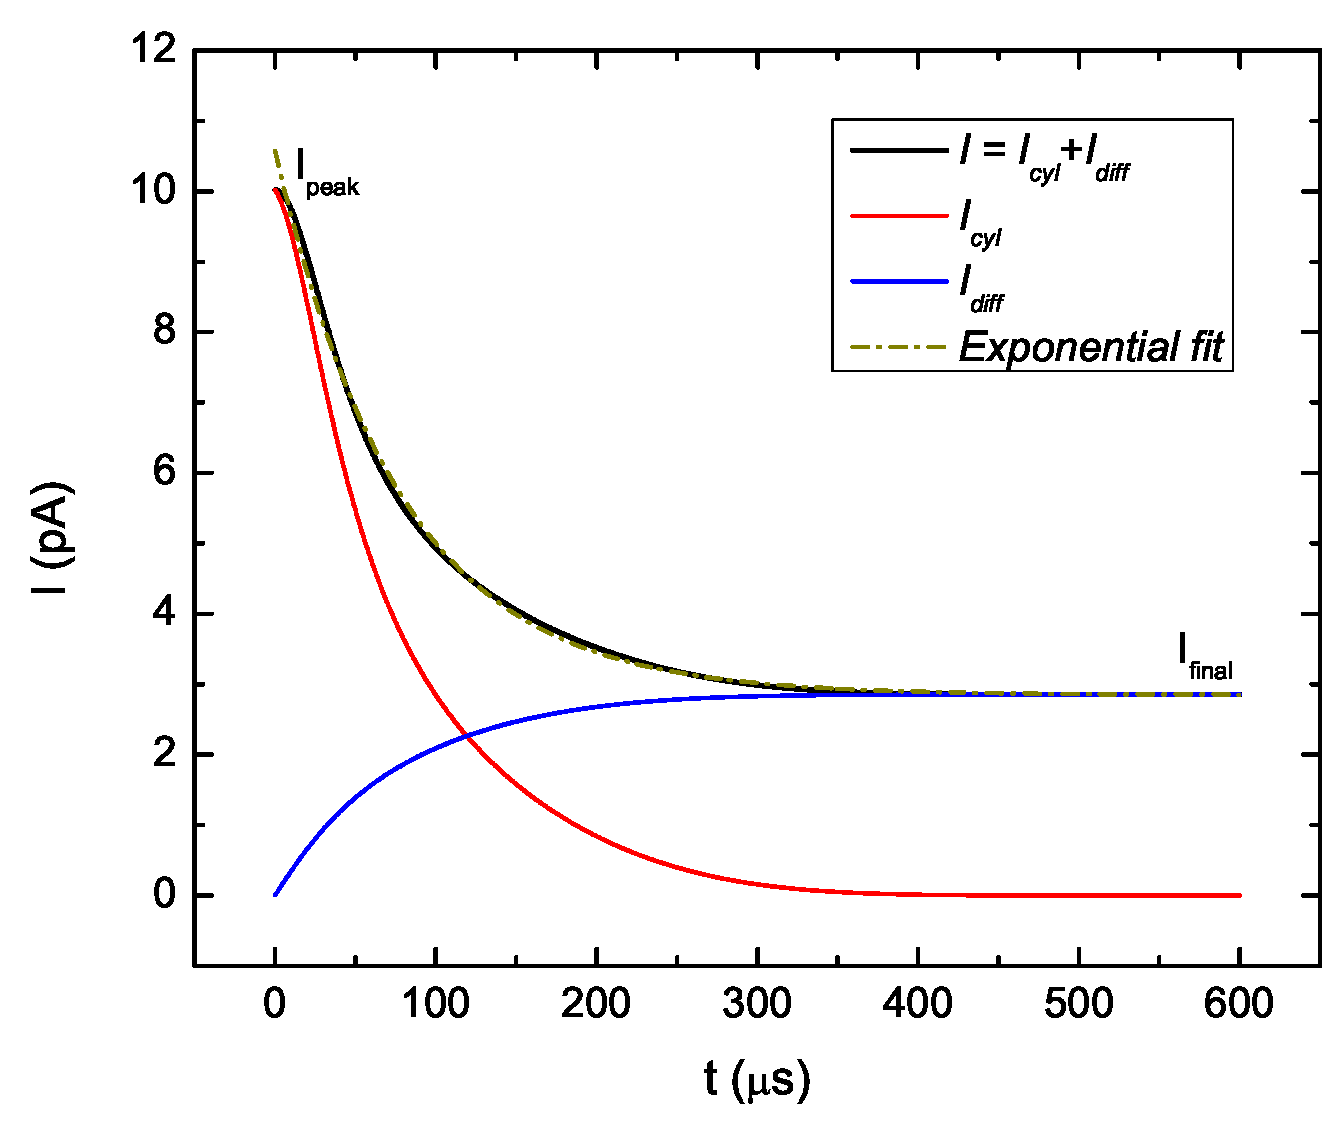
\includegraphics[width=0.7\linewidth]{pics/currmea/TypicalCurrentProfile.eps}
    \caption{A plot of the behavior of the modeled current $I(t)$ and its separate contributions $I_{diff}$ and $I_{cyl}$ as a function of time, at $s_0=1$. An exponential decay is plotted as a dashed line. The maximum current is indicated with $I_{peak}$ and the steady-state current with $I_{final}$.}
    \label{fig:TypicalCurrentProfile}
\end{figure}
In this plot, the current has been separated in these two contributions (similarly as discussed before for the number of atoms in the core region). The diffusion current $I_{diff}(t) = e r_i N_{core}^{(diff)}(t)$ increases with time, up to a final value. In contrast, the current due to atoms starting in the cylinder $I_{cyl}(t) = e r_i N_{cyl}^{(diff)}(t)$ decreases to zero with time. The total current $I(t) = I_{diff}(t) + I_{cyl}(t)$ typically resembles an exponential decay with a time constant $\tau$, with an initial maximum $I_{peak}$ and a steady level $I_{final}$.

It is also useful to define the average current $\overline{I}$, the peak current $I_{peak}$, the final current $I_{final}$ and the charge per pulse $Q$:
\begin{equation}
    \overline{I} = \frac{1}{t_{cycle}} \int_0^{t_i}{I(t)dt},
    \label{eq:avg_current}
\end{equation}
\begin{equation}
    I_{peak} = \mbox{max} \left(I(t)\right),
    \label{eq:peak_current}
\end{equation}
\begin{equation}
    I_{final} = I(t_i),
    \label{eq:final_current}
\end{equation}
\begin{equation}
    Q = \int_0^{t_i}{I(t)dt}.
    \label{eq:charge}
\end{equation}

Figure \ref{fig:TypicalAverageCurrent} shows a typical two-dimensional plot of the average current as a function of the ionization time on the horizontal scale and of the loading time on the vertical scale.
\begin{figure}[tbh!]
    \centering
        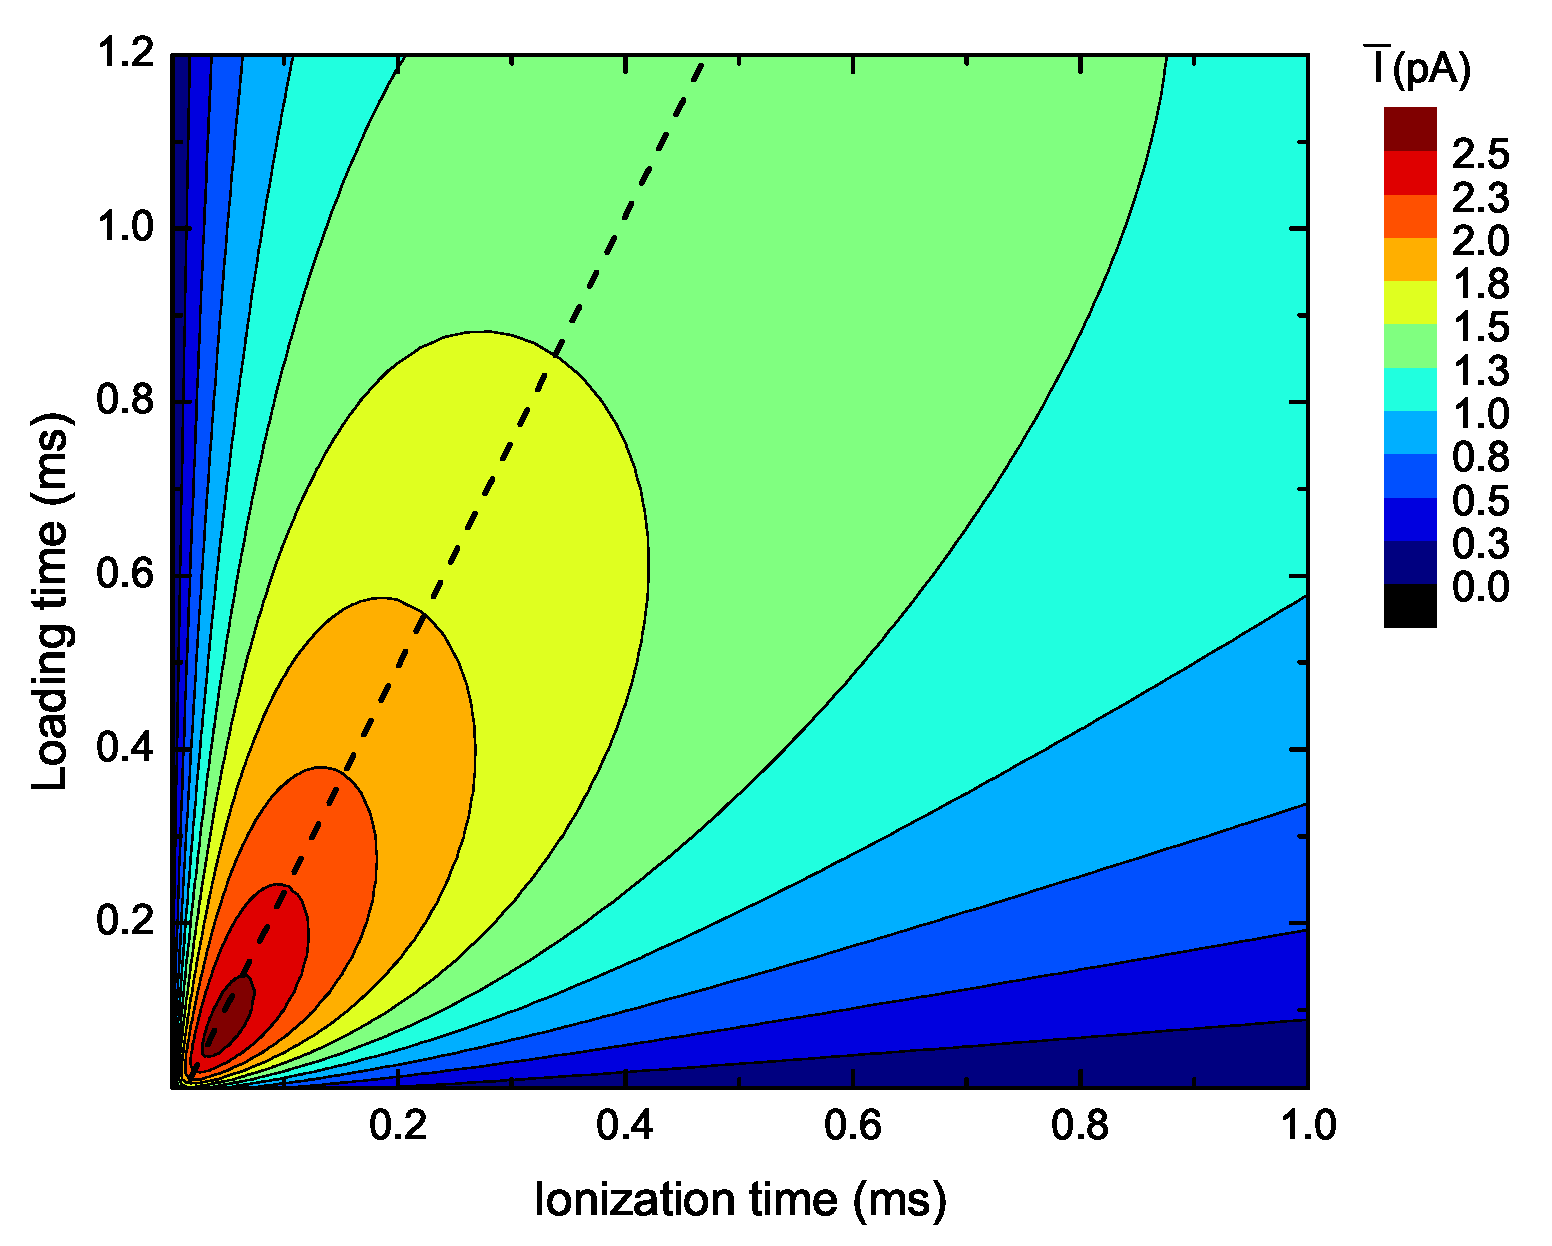
\includegraphics[width=0.7\linewidth]{pics/currmea/TypicalAverageCurrent.eps}
    \caption{Behavior of the modeled average current (color scale) versus the loading time (vertical axis) and the ionization time (horizontal axis), at $s_0=1$. There is a clear optimum for $t_l \approx 100$ $\mu$s and $t_i \approx 50$ $\mu$s. The dashed line highlights the optimal ratio between loading and ionization times for the highest obtainable current.}
    \label{fig:TypicalAverageCurrent}
\end{figure}
A clear maximum is $\overline{I}=2.5$ pA obtained with $t_i \approx 50$ $\mu$s and $t_l \approx 100$ $\mu$s. The loading time is twice the ionization time, corresponding to $\langle N \rangle = N_{\infty}/2$, from equation (\ref{eq:aveN}). From the type of plot shown in figure \ref{fig:TypicalAverageCurrent}, a few important quantities can be extrapolated. The first one is simply the maximum of the average current $\overline{I}_{max}$. Also, for a given ionization time for which the average current is maximized there is an optimum. A curve is drawn as a dashed line in figure \ref{fig:TypicalAverageCurrent} that indicates the dependence. To first order, the curve is a straight line that can be characterized by its slope. We extract the slope by linear regression. The slope $\rho=t_l/t_i$ represents the optimal ratio between the loading and the ionizing times, and is related to the optimal duty cycle $D$ at which the highest current is obtained. The duty cycle is given by
\begin{equation}
    D=\frac{t_i}{t_{cycle}} \cong \frac{1}{\rho + 1},
    \label{eq:Dcycle}
\end{equation}
where the 10 $\mu$s in the definition of $t_{cycle}$ have been ignored since $t_{cycle} \gg 10$ $\mu$s.

\section{Experimental results} \label{sec:expres}
The goal of the measurements is the optimization of the extracted current and the verification of the model described in section \ref{sec:model}. In order to achieve these objectives, first the parameters of the model have been experimentally determined: the temperature $T_s$ of the trapped atoms, the loading rate of the MOT $R_L$ and the lifetime of the MOT with trapping laser beams turned on ($\tau_M$) and while they are turned off ($\tau'_M$). Table \ref{tab:measPar} summarizes the measured parameters for the model presented in section \ref{sec:model}.
\begin{table}[ht]
	\caption{\label{tab:measPar} Measured parameters of the model.}
	\begin{center}
		\begin{tabular}{| l | l | l |  }
			\hline
			Parameter & Symbol & Value \\ \hline
			Source temperature & $T_s$ & $(230 \pm 30)$ $\mu$K \\
			Loading rate & $R_L$ & $(12 \pm 1) \times 10^8$ s$^{-1}$ \\ 
			MOT Lifetime (trap on) & $\tau_M$ & $(180 \pm 5)$ ms \\ 
			MOT Lifetime (trap off) & $\tau'_M$ & $(71 \pm 6)$ ms \\
			\hline
		\end{tabular}
	\end{center}
\end{table}

\subsection{Parameters of the model}
\label{sec:param}
{\bf Trap temperature.} The trap temperature is an important parameter in our model, as it affects the diffusion between the core region and the rest of the MOT, as well for the expansion of the MOT itself while the trapping lasers are turned off. After the trapping laser beams are turned off at $t=0$, the MOT expands according to the relation
\begin{equation}
    \sigma_M^2(t_e) = \sigma_M^2(0) + \left(\frac{k_b T_s}{m}\right) t_e^2,
    \label{eq:sigma_MOT}
\end{equation}
where $k_b$ is Boltzmann's constant \cite{Weiss_JB_89}. 
The MOT cameras are triggered to measure the fluorescence light emitted by the trapped atoms at a variable delay time up to 8~ms after the trapping lasers are turned off (at $t=0$). The trapping laser beams are flashed on for 250 $\mu$s to produce the fluorescence light. The \textit{rms}-radii of the MOT are calculated by fitting the images with a 2D-Gaussian. The square of the \textit{rms}-radius of the MOT is plotted versus the square of the expansion time in figure \ref{m1}.
\begin{figure*}[tbh!]
	\subfloat[Source temperature\label{m1}]{\includegraphics[width=0.48\linewidth]{pics/currmea/Temperature}}
	\hfill	
	\subfloat[Loading rate\label{m2}]{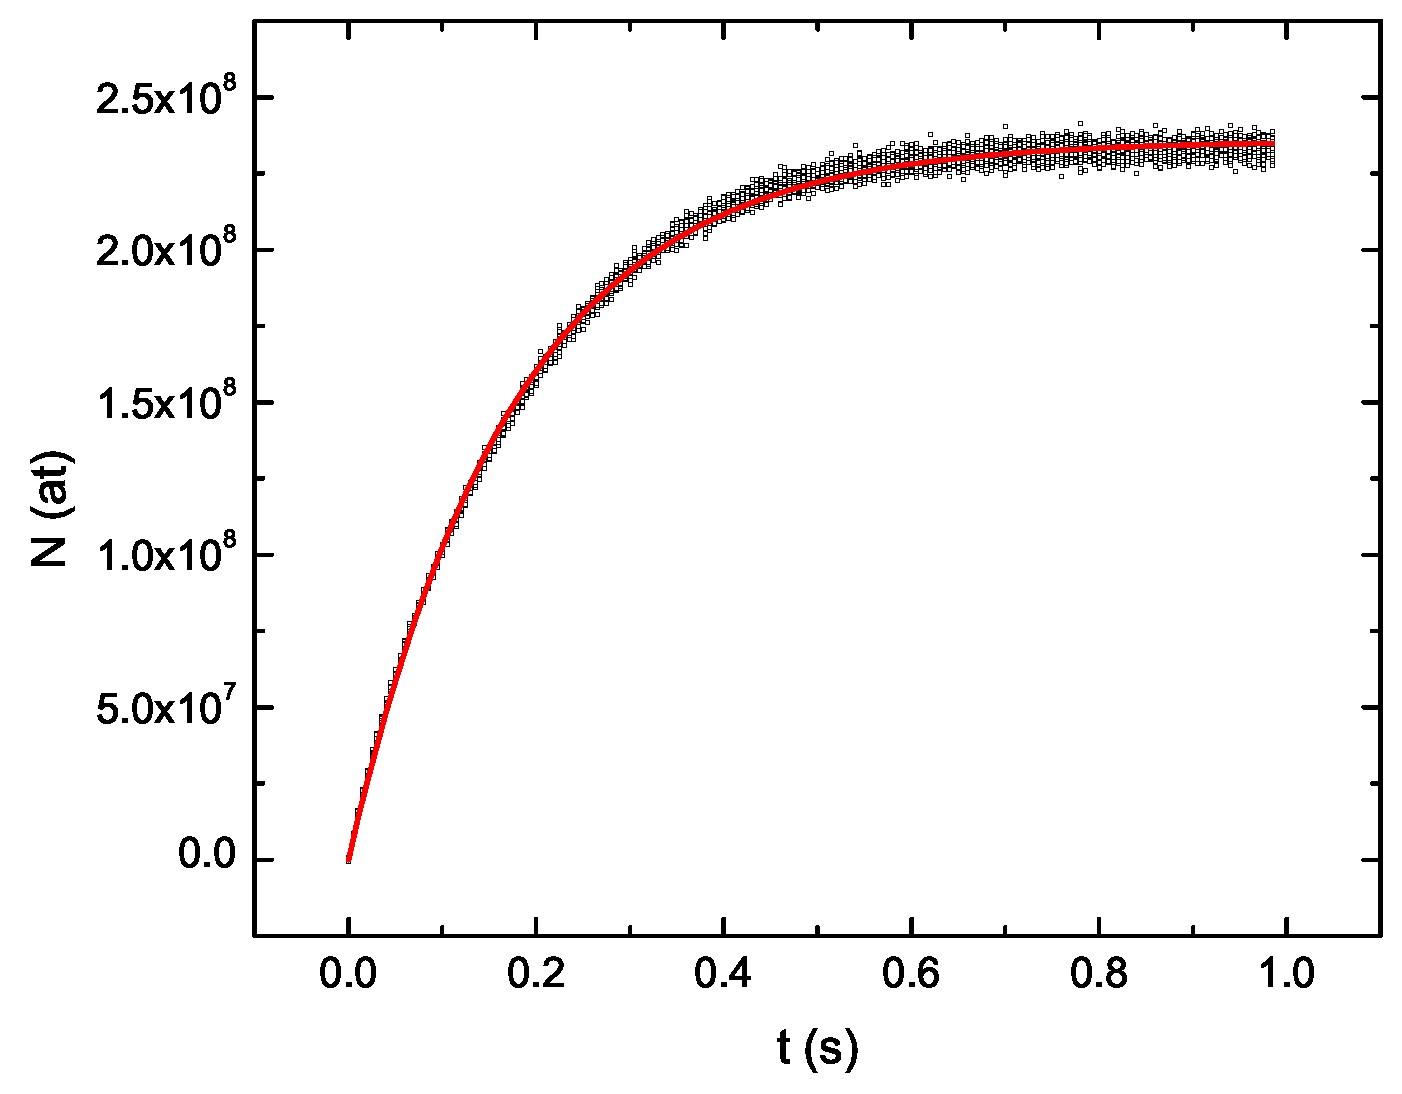
\includegraphics[width=0.48\linewidth]{pics/currmea/LoadingRate}}
	\\
	\subfloat[Number of atoms\label{m3}]{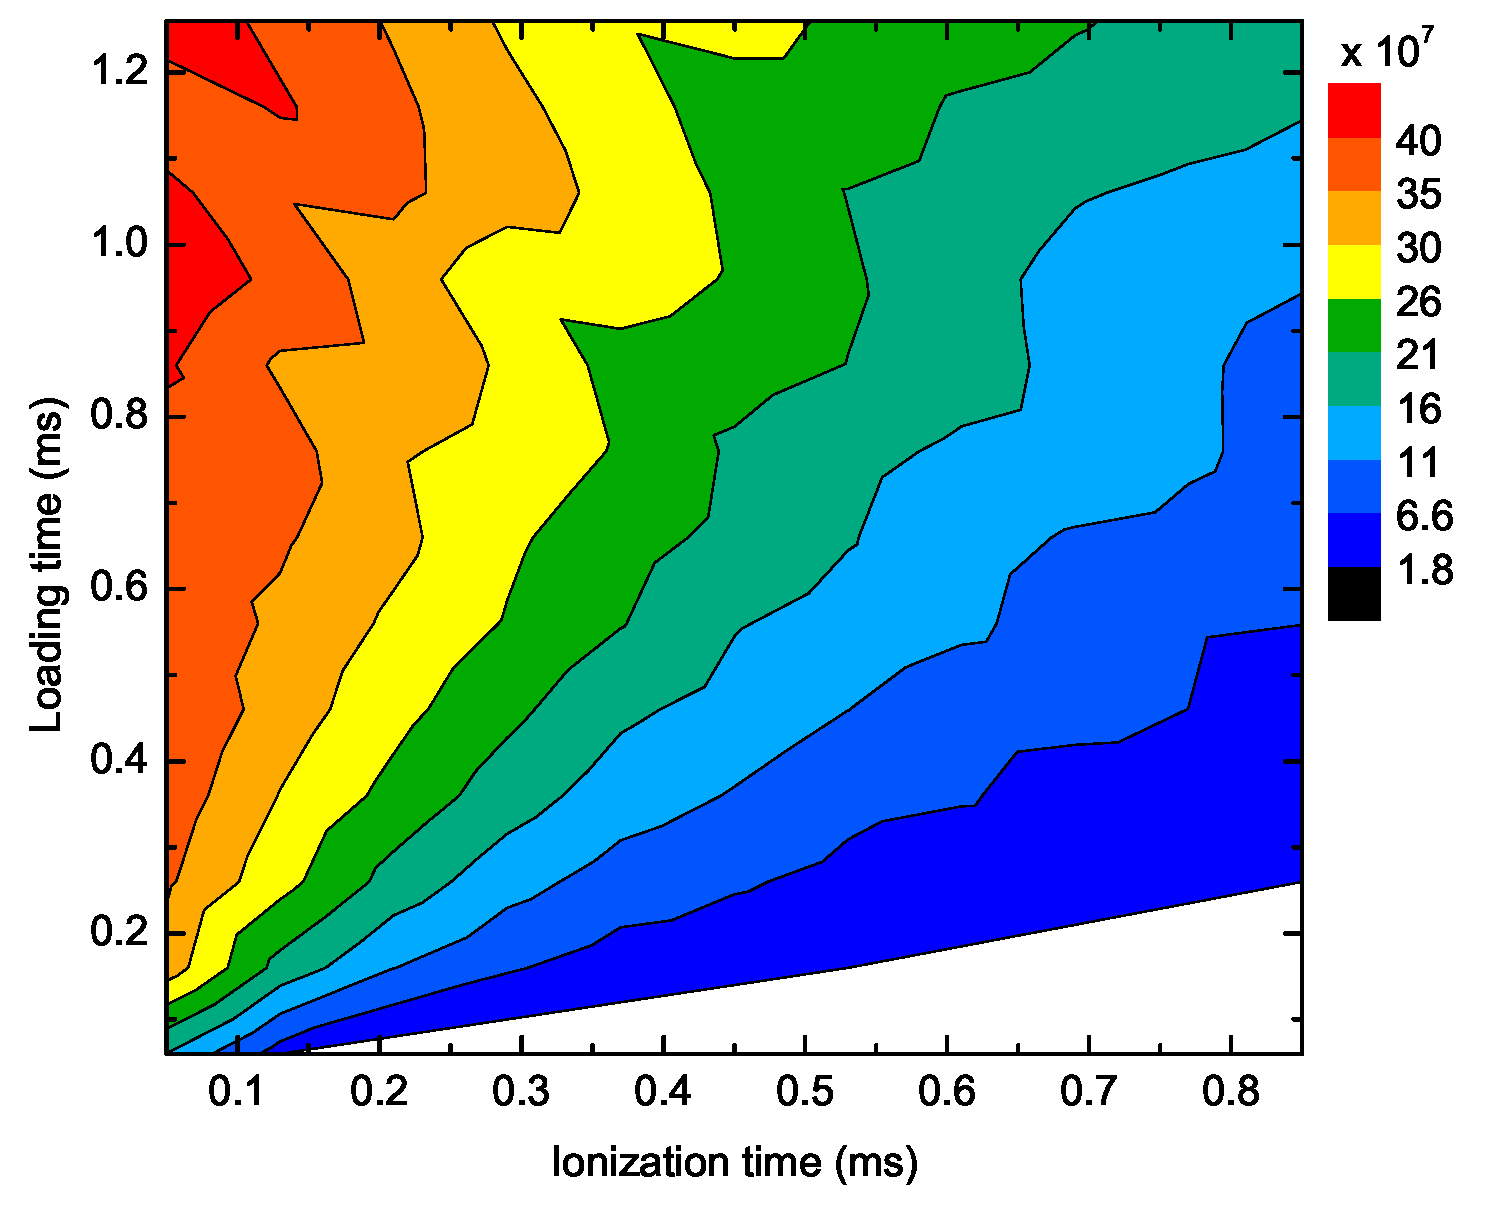
\includegraphics[width=0.48\linewidth]{pics/currmea/NumberAtoms2DPlot}}
	\hfill	
	\subfloat[Number of atoms\label{m4}]{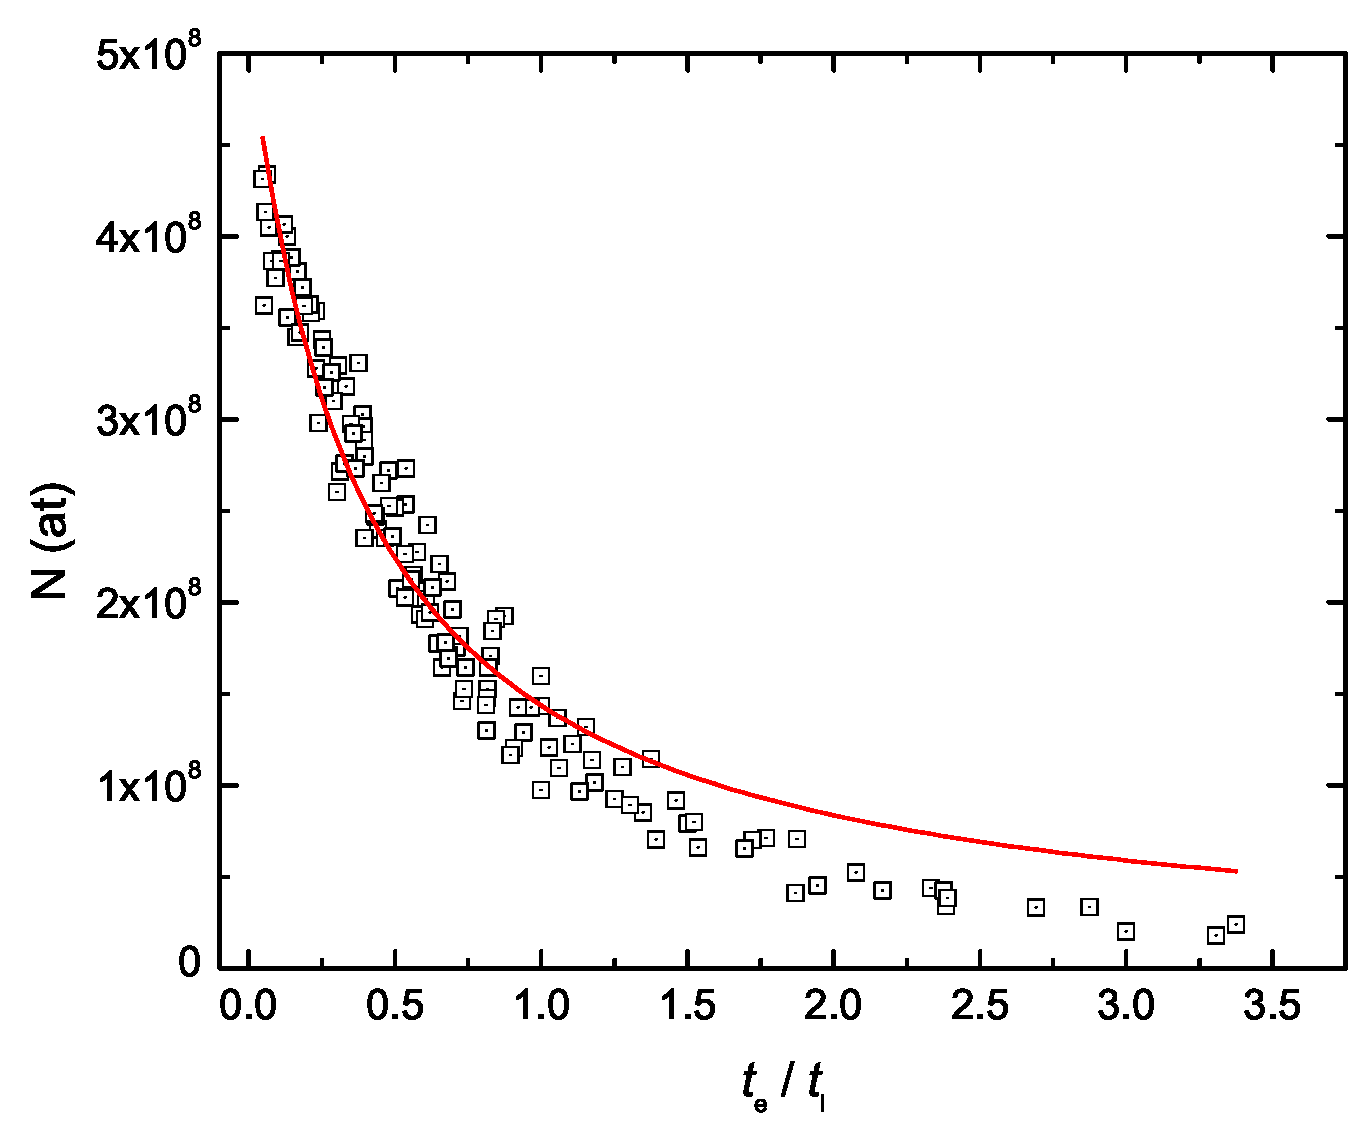
\includegraphics[width=0.48\linewidth]{pics/currmea/NumberAtomsCombinedXaxis}}	
	\caption{In panel (a), a typical result of the source temperature measurements is shown. The square of the \textit{rms}-radii of the MOT are plotted versus the expansion time squared. In panel (b), the number of atoms in the MOT while loading the MOT is plotted versus the time. The data is fitted with equation (\ref{eq:RL_rate}) in order to determine the loading rate of the MOT and its lifetime. In panel (c), a contour plot of the number of atoms versus the ionization time and the loading time is shown. In panel (d), a plot of the number of atoms in the MOT versus the ratio of the expansion and the loading times is shown. The data is fitted with equation (\ref{eq:aveN}) in order to determine the lifetime with trapping laser beams off. \label{fig:parameas}}
\end{figure*}
The trap temperature, determined from a fit of equation (\ref{eq:sigma_MOT}) to the data, is $(230 \pm 30)~\mu$K, not far from the Doppler temperature $T_D = 143$ $\mu$K of the $^{85}$Rb transition. The uncertainty in the extracted temperature reflects the degree of agreement between data sets.\\

\noindent {\bf Loading rate and lifetime.} Starting with an empty trap, at $t=0$ the trapping laser beams are turned on and the amount of fluorescent light emitted by the trapped atoms is monitored with two calibrated CCD cameras. The exposure time of the cameras is 5 ms and they are triggered at intervals of 40 ms and different measurement sweeps were shifted in steps of 5 ms. The measurement is repeated 25 times for sufficient statistical accuracy. The pixel counts of one camera image are then summed and the number of atoms is calculated. Figure \ref{m2} shows a typical result of the experiment. The result is fitted with equation (\ref{eq:RL_rate}), giving $\tau_M = (180 \pm 5)$~ms and $R_L = (12 \pm 1) \times 10^8$~atoms/s. The 10~\% accuracy reflects the degree of agreement between the two cameras.\\

\noindent {\bf Number of Atoms.} The average number of trapped atoms $\langle N \rangle$ under continuous cycling was determined with the CCD cameras for a range of loading and ionization times. The measured number of atoms is plotted versus the ionization time and the loading time in figure \ref{m3}. The contour lines are in first approximation straight lines passing through the origin. Therefore the number of trapped atoms is a function of the combined variable $t_e/t_l$ and a plot is shown in figure \ref{m4}. The solid line is a fit according to equation (\ref{eq:aveN}). The fit follows the overall trend but it is too high for large $t_e/t_l$. However this deviation is not important since the optimum for the current occurs at $t_e/t_l < 1$, where there is a good agreement. Finally, the last missing parameter of the model can be calculated. From the fit, it follows $\zeta = 2.5 \pm 0.1$ and $\tau'_M = (71 \pm 6)$ ms, using the measured value of $\tau_M = (180 \pm 5)$ ms measured previously in this section.\\

\subsection{Typical current signal}
\label{sec:typcurrent}
This section discusses the temporal behavior of the measured current pulses. Two measurements have been selected and are shown in figure \ref{fig:signals}: the first for a large saturation parameter $s_0=4$ and $t_i=130$ $\mu$s, and the second one for a smaller saturation parameter $s_0=0.2$ and $t_i=770$ $\mu$s. The loading time is $t_l=250$ $\mu$s in both cases.
\begin{figure*}[tbh!]
	\subfloat[$s_0 = 4$\label{c1}]{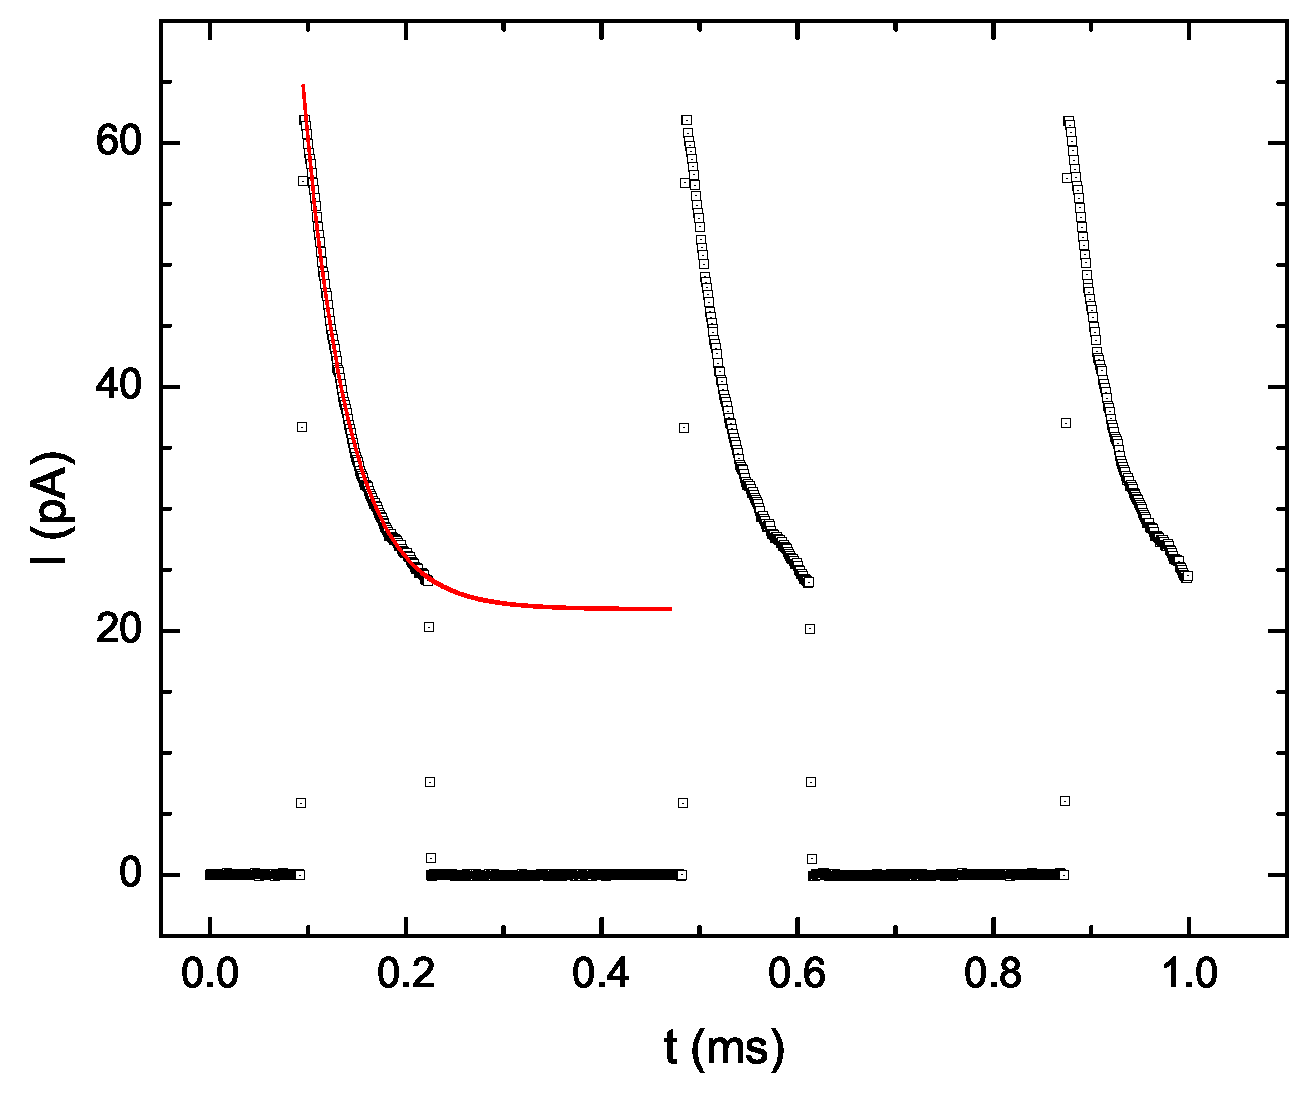
\includegraphics[width=0.48\linewidth]{pics/currmea/CurrentVsTimeS=4}}
	\hfill	
	\subfloat[$s_0 = 0.2$\label{c2}]{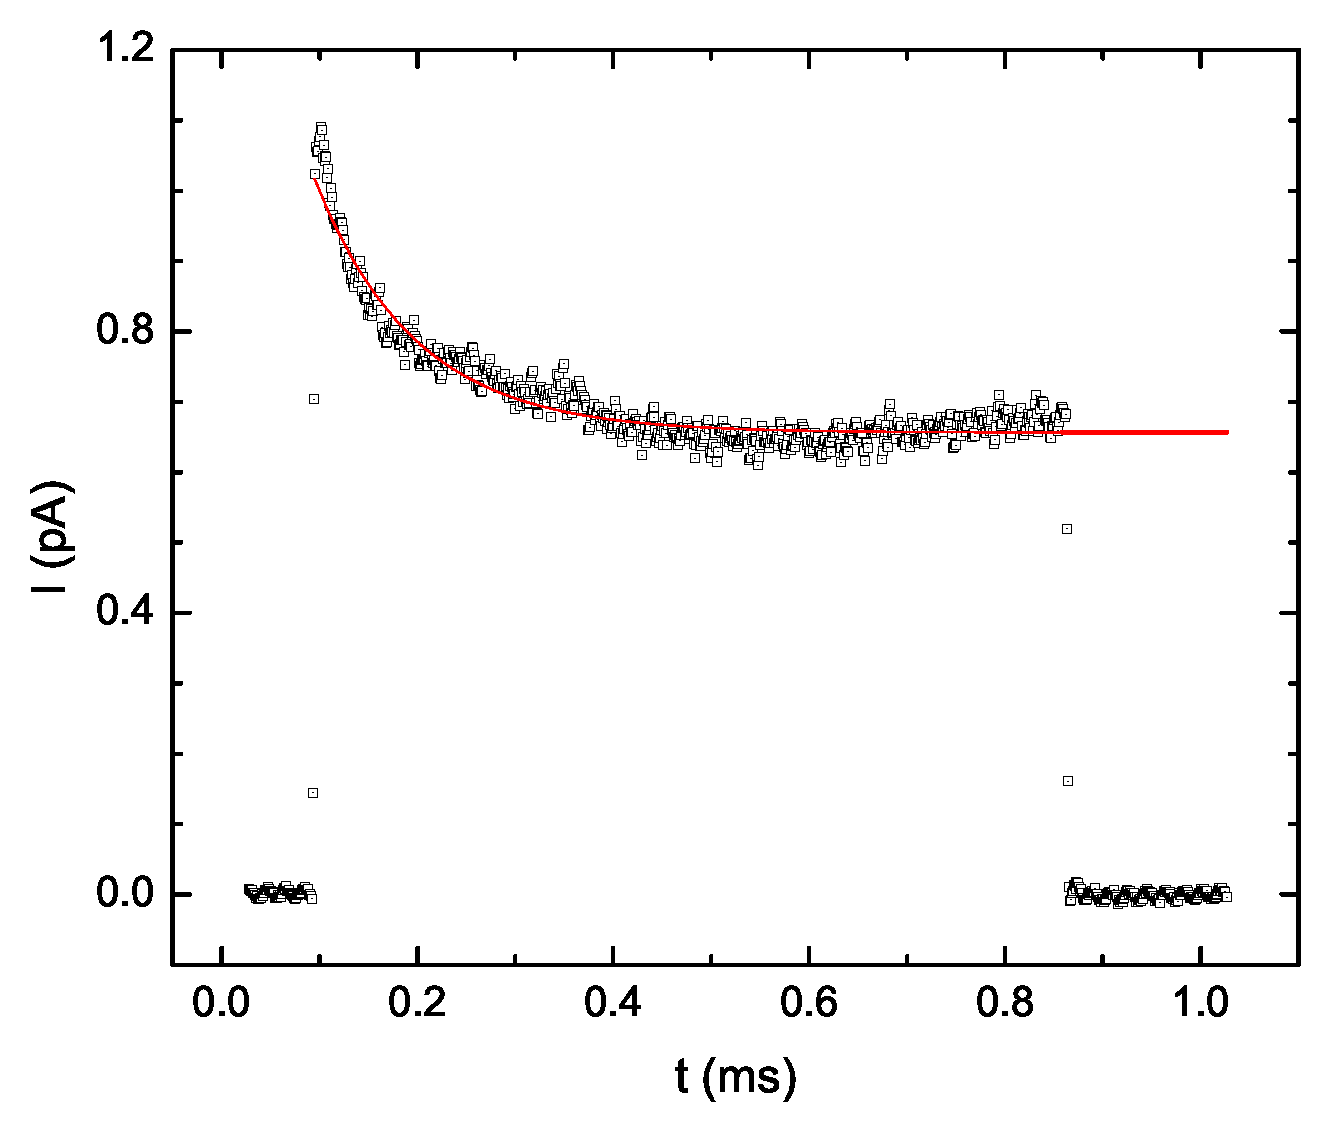
\includegraphics[width=0.48\linewidth]{pics/currmea/CurrentVsTimeS=0,2}}
	\caption{Current plotted versus time for two values of the saturation parameter of the excitation laser beam. The solid line is an exponential fit of the data. The peak current is much larger for $s_0=4$ as well as the ratio $I_{peak}/I_{final}$.\label{fig:signals}}
\end{figure*}
The two plots show a number of differences. One of these is the magnitude of the peak current: $I_{peak}=62$ pA in figure \ref{c1} against $I_{peak}=1.1$ pA in figure \ref{c2}. This is partly caused by the difference in excited state fraction ratio $f(4,0)/f(0.2,0) = 4.8$, but the difference in the number of trapped atoms is more important. In figure \ref{c2}, the ionization time is about 3 times longer than the loading time, while in figure \ref{c1} this is a factor of 2 shorter. From figure \ref{m4}, this corresponds to $\langle N \rangle= 2.5 \times 10^8$ atoms and $2.5 \times 10^7$ atoms respectively. The two effects combined change the peak current by a factor 48, which is comparable with the difference in the peak current in the two measurements (a factor $\approx$~56).

The second difference is the ratio between the peak and the final current $I_{peak}/I_{final}$. This ratio is 2.8 for $s_0=4$ since the final current is $I_{final}=22$ and 1.4 for $s_0=0.2$ since $I_{final}=0.7$ pA. This difference can be explained with the model and it is caused by the different $s_0$ as shown in figure \ref{fig:CompDiffCyl}, where ratios of 3.9 and 2.2 are respective calculated at the same $s_0$. The measured values are both a factor 1.5 lower, possibly due to local variation of the MOT density.

Finally, the currents resemble quite well an exponential decay, with time constants of $\tau = 45$ $\mu$s in figure \ref{c1} and $\tau = 102$ $\mu$s in figure \ref{c2}, drawn as solid lines. The value for figure \ref{c1} is somewhat uncertain because the final current level is not reached yet due to the short $t_i$. Nevertheless, the time constant clearly depends on $s_0$ as predicted by the model (see figures \ref{fig:Ncorecyl} and \ref{fig:Ncorediff}).

\subsection{Moving the ionization laser beam}
\label{sec:verify}
The model predicts that the atoms that are ionized have been pushed into the core region by the excitation laser beam. Therefore the total charge created can be increased by moving the ionization laser beam away from the center of the MOT, in the positive $z$-direction (see figure \ref{fig:setup}). In this way the excitation laser cylinder (see figure \ref{fig:cylGeo}) can be made longer, increasing the number of atoms it contains. However, for larger displacements the current will be reduced once outward diffusion becomes important. In addition, the initial current will be reduced because the ionization laser beam is no longer in the center of the MOT (where the density is maximum). In order to verify this picture, an experiment is performed where the current is measured for several $z$-positions of the ionization laser beam. This experiment uses a long ionization time $t_i = 900$ $\mu$s, so that the current will nearly reach its final value, a very long loading time of $t_l = 5$ ms and $s_0=4$. Here $\Delta z > 0$ corresponds to a displacement of the ionization laser spot in the same direction as the atoms are pushed.
 
For several values of $\Delta z$ (in units of $\sigma_M \approx 0.8$ mm), calculated and measured current profiles have been plotted in figure \ref{fig:dispIoniz}. 
\begin{figure*}[tbh!]
\subfloat[model\label{d1}]{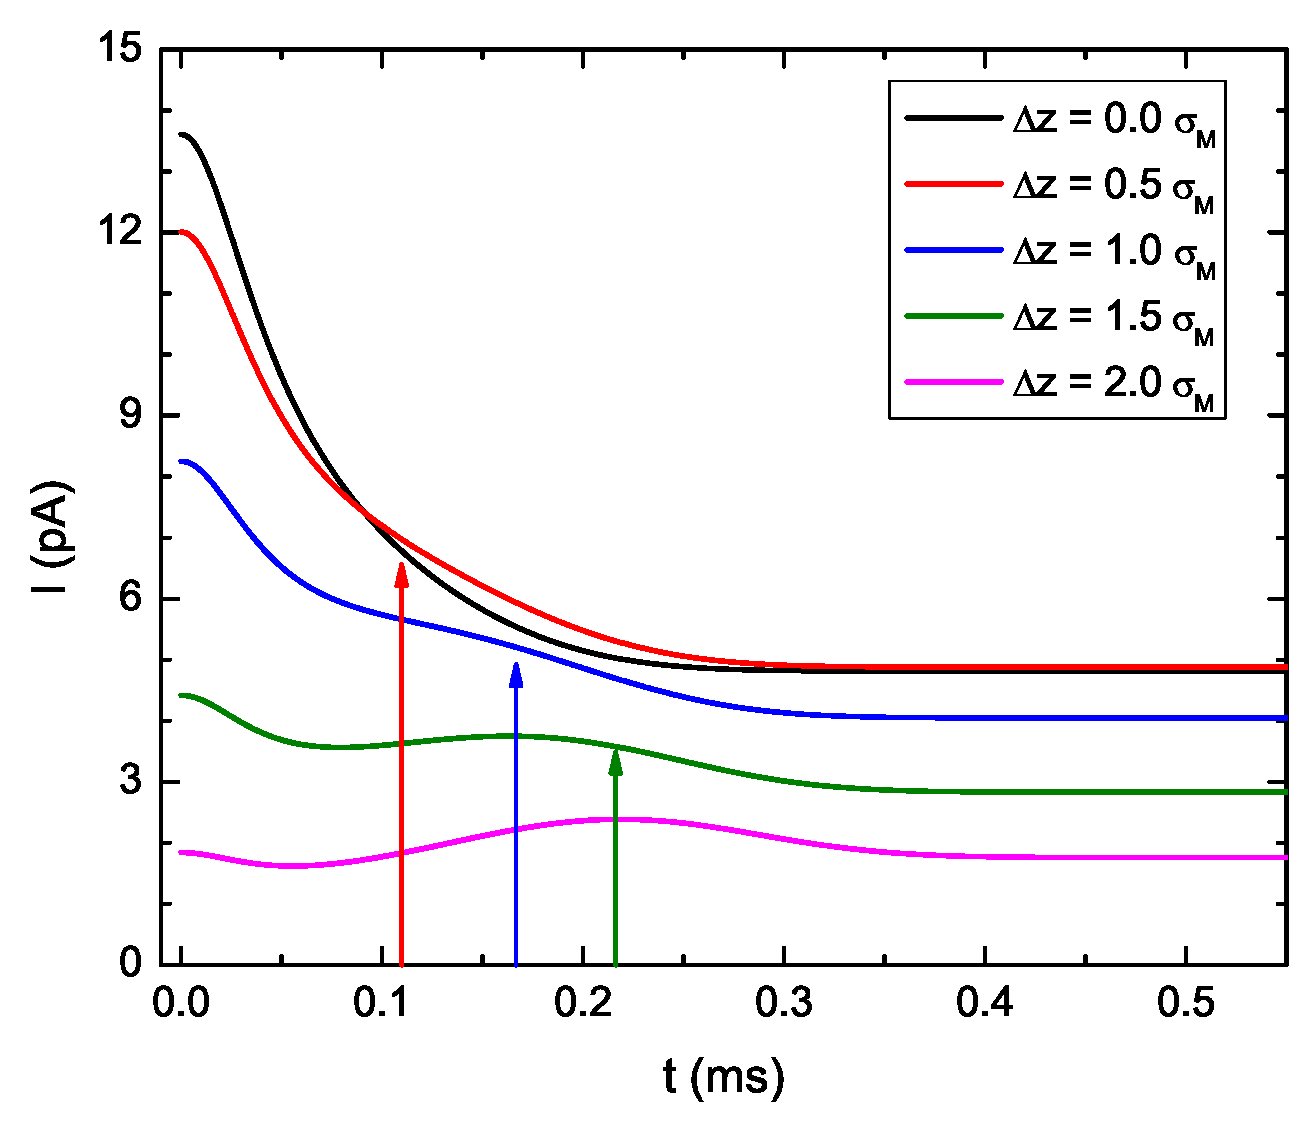
\includegraphics[width=0.48\linewidth]{pics/currmea/IonisationPositionModeledCurrent}}
	\hfill		
	\subfloat[measurement\label{d2}]{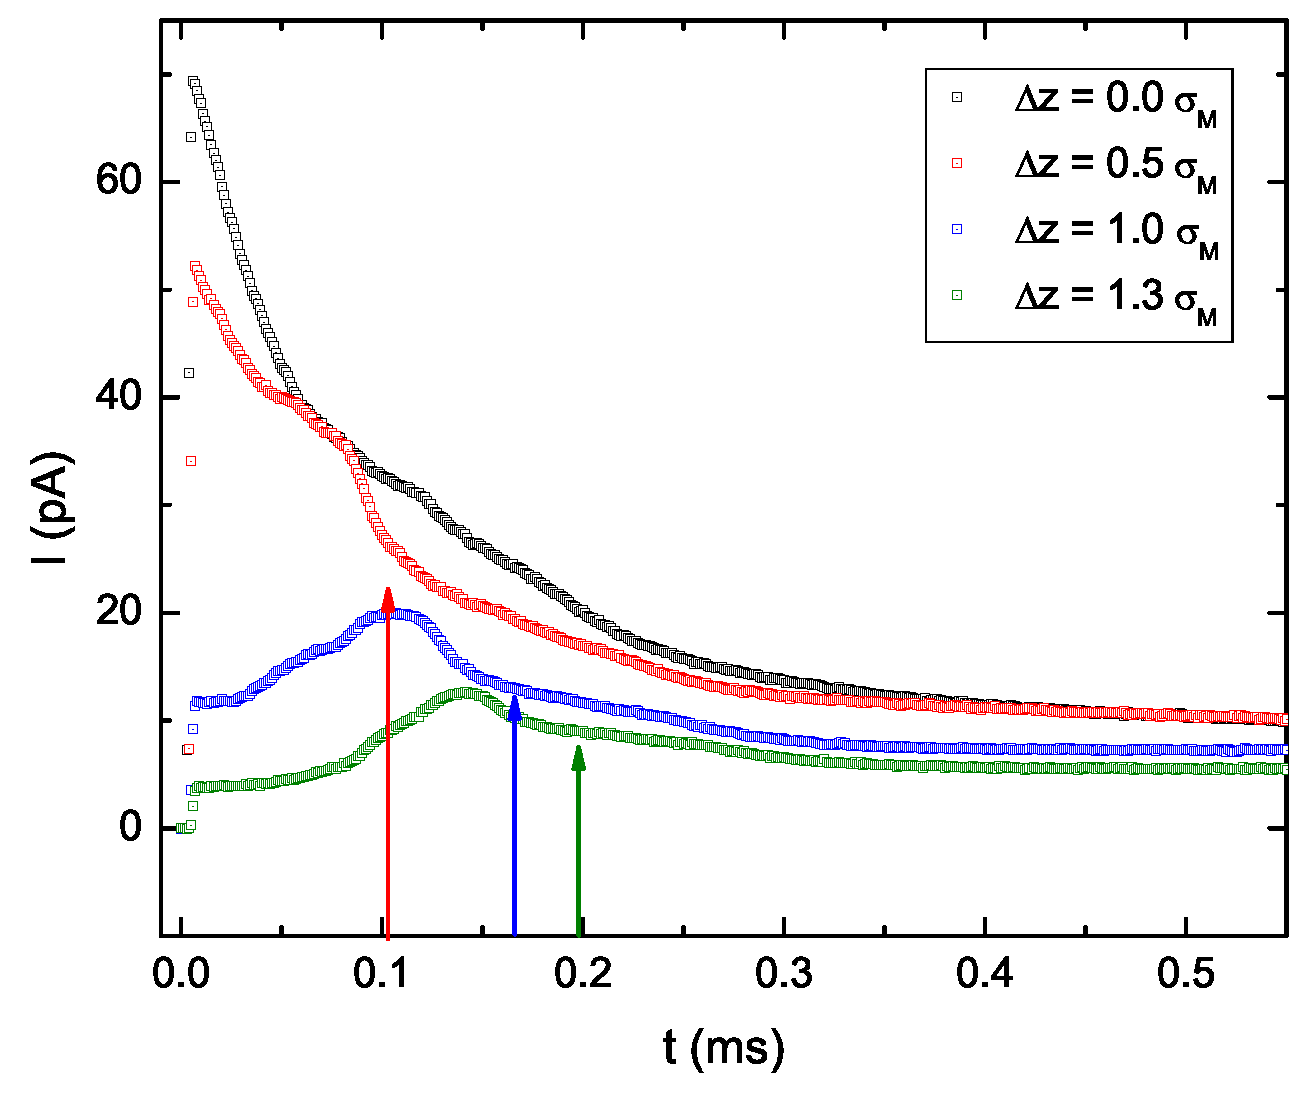
\includegraphics[width=0.48\linewidth]{pics/currmea/IonisationPositionMeasuredCurrent}}
	\caption{Current behavior if the ionization laser is shifted relative to the position where the initial current is maximal at the center of the MOT ($\Delta z = 0$). The figures compare the model predictions and the experimental results for several displacements $\Delta z$. The decay of the current is slower for larger shifts, and a ``bump'' appears on top of the ``exponential decay''. A colored arrow indicates the time when the ``bump'' occurs according to the simple approximation (see text).\label{fig:dispIoniz}}
\end{figure*}
For the calculations, a shifted density term 
\begin{equation}
    n(z)=n_c e^{\left( -(z-\Delta z)^2 / {2 \sigma_M^2} \right)},
    \label{eq:shiftn}
\end{equation}
is used instead of the density at $z=0$ of equation (\ref{eq:density}). Comparing the two figures, a number of similarities are observed. In both cases, the initial current decreases when $\Delta z$ is increased, because the density at the ionization laser position decreases. Also, in both cases, the current gets an extra "bump": it no longer matches an exponential decay, but has a broad peak added to it. The time at which this peak occurs increases with $\Delta z$. It is approximately given by the time needed for an atom to be pushed over the distance $\Delta z$, the solution of equation (\ref{eq:distance}). This gives $t_{peak} = 111$ $\mu$s for $\Delta z= 0.5~\sigma_M$, $t_{peak} = 168$ $\mu$s for $\Delta z = \sigma_M$ and $t_{peak} = 215$ $\mu$s for $\Delta z = 1.5~\sigma_M$, for the model. The first three peak positions based on this approach have been marked with coloured arrows in figure \ref{fig:dispIoniz}. This simple approach does not take into account effects like outward diffusion and increasing of the Doppler shifts, which both will make the real peak occur earlier. Also, because these peaks are superimposed on the exponential decay, the actual peak positions will seem to occur earlier. Nevertheless, it gives quite a good approximation of the behavior in both the model and the experiment.
 
Next, both the model and the experiment show that shifting the ionization laser too far, will result in a lower current for the whole time the ionization laser beam is turned on, compared to $\Delta z =0$. This is the case for $\Delta z \geq \sigma_M$ both in the modeled current and in the experiment. Clearly, the outward diffusion and decreasing excited state fraction for larger time of flight, prevent the extra atoms in the cylinder from being ionized. For smaller shifts, $\Delta z = 0.5~\sigma_M$, both the model and the experiment show a slightly larger final current, which can be desirable for extremely long pulses, where only the final level of the current is relevant. For shifts $0 < \Delta z < 0.5~\sigma_M$ an optimum occurs, where also for shorter ionization times the obtained current is larger than without the shift.

One aspect where the model and experiment do not agree, is how much the initial current decreases when $\Delta z$ is increased. This is probably caused by deviations of the number density from strict Gaussian behavior, observable as asymmetries present in the shape of the MOT. 

\subsection{Current optimization measurement}
\label{sec:currentmea}
The main parameters of the model have been measured in section \ref{sec:param} and the model has been verified in section \ref{sec:verify}. The main goal of this paper is to optimize the extracted current. The average current, equation (\ref{eq:avg_current}), is measured while the loading and the ionization times are varied. This results in a contour plot similar to the one presented in figure \ref{fig:TypicalAverageCurrent}. These measurements have been performed at different values of the excitation laser beam saturation parameter and ionization laser beam power. Every set of measurements is performed in a random order to prevent drift from influencing the results. The measurement time varies between 30 and 60 minutes depending on the number of steps. Typically, the ionization power energy is $P_i=46$~mW, unless specified.\\

\noindent {\bf Saturation parameter dependence.} The saturation parameter is changed by varying the power of the excitation laser beam with the use of an AOM. Figure \ref{fig:smallVdiffs} shows two scans performed at $s_0 = 1$ and $s_0=12$. In both of the scans, $t_l$ is incremented in steps of 100 $\mu$s between 50 and 1250 $\mu$s and $t_i$ ranges between 50 and 850 $\mu$s in steps of 80 $\mu$s, a total of 143 points. 
\begin{figure*}[tbh!]
	\subfloat[$s_0 = 1$\label{s1}]{\includegraphics[width=0.52\linewidth]{pics/currmea/2DPlotS=1}}
	\hfill	
	\subfloat[$s_0 = 12$\label{s2}]{\includegraphics[width=0.45\linewidth]{pics/currmea/2DPlotS=12}}
	\caption{Contour plots of the average current versus the loading time (vertical axes) and the ionization time (horizontal axis), for $s_0=1$ and $s_0=12$. The color scale is the same for both of the plots. The dashed line highlights the slope $\rho$ at which the highest average current occurs. A black dot marks the maximum of the average current. The average current is larger for a higher $s_0$ and the same conclusion is valid for the slope.\label{fig:smallVdiffs}}
\end{figure*}
These plots strongly resemble the one from the model shown in figure \ref{fig:TypicalAverageCurrent}, especially the one at $s_0=12$. In general, a higher saturation parameter is beneficial for increasing the average current. The maximum average current is marked with a black dot in the plots. The average current is about a factor of two higher, $\overline{I} \approx 8.2$~pA at $s_0=12$ compare to $\overline{I} \approx 3.8$ pA at $s_0=1$, and this is mainly caused by the higher excited state fraction: $f(12,0)/f(1,0) \approx 1.8$. A stronger ``pushing effect'' is also important, since it leaves less time for the atoms to diffuse out of the cylinder.\\

It follows from the plot that it is better to ionize for a short time, going for a higher repetition rate rather than a low one. The optimum ratio $\rho$ where the maximum of the average current occurs is drawn as a dashed line in the two figures: $\rho= 2.3$ for $s_0=12$ and $\rho = 1.4$ for $s_0=1$. Clearly it becomes beneficial to use a shorter ionization phase for a higher saturation parameter and this is a direct consequence of the larger ratio between the peak and the final current already discussed in Subsection \ref{sec:typcurrent}.
The maximum average current measured in all the experiments is $(13 \pm 1)$ pA, obtained at a duty cycle of 36\%. The maximum peak current measured is $(88 \pm 5)$ pA. The uncertainty of the current is related to the calibration of the MCP.

The contour plot of the charge per pulse for $s_0=12$ is plotted in figure \ref{fig:charge2Dplot}.
\begin{figure}[tbh!]
    \centering
        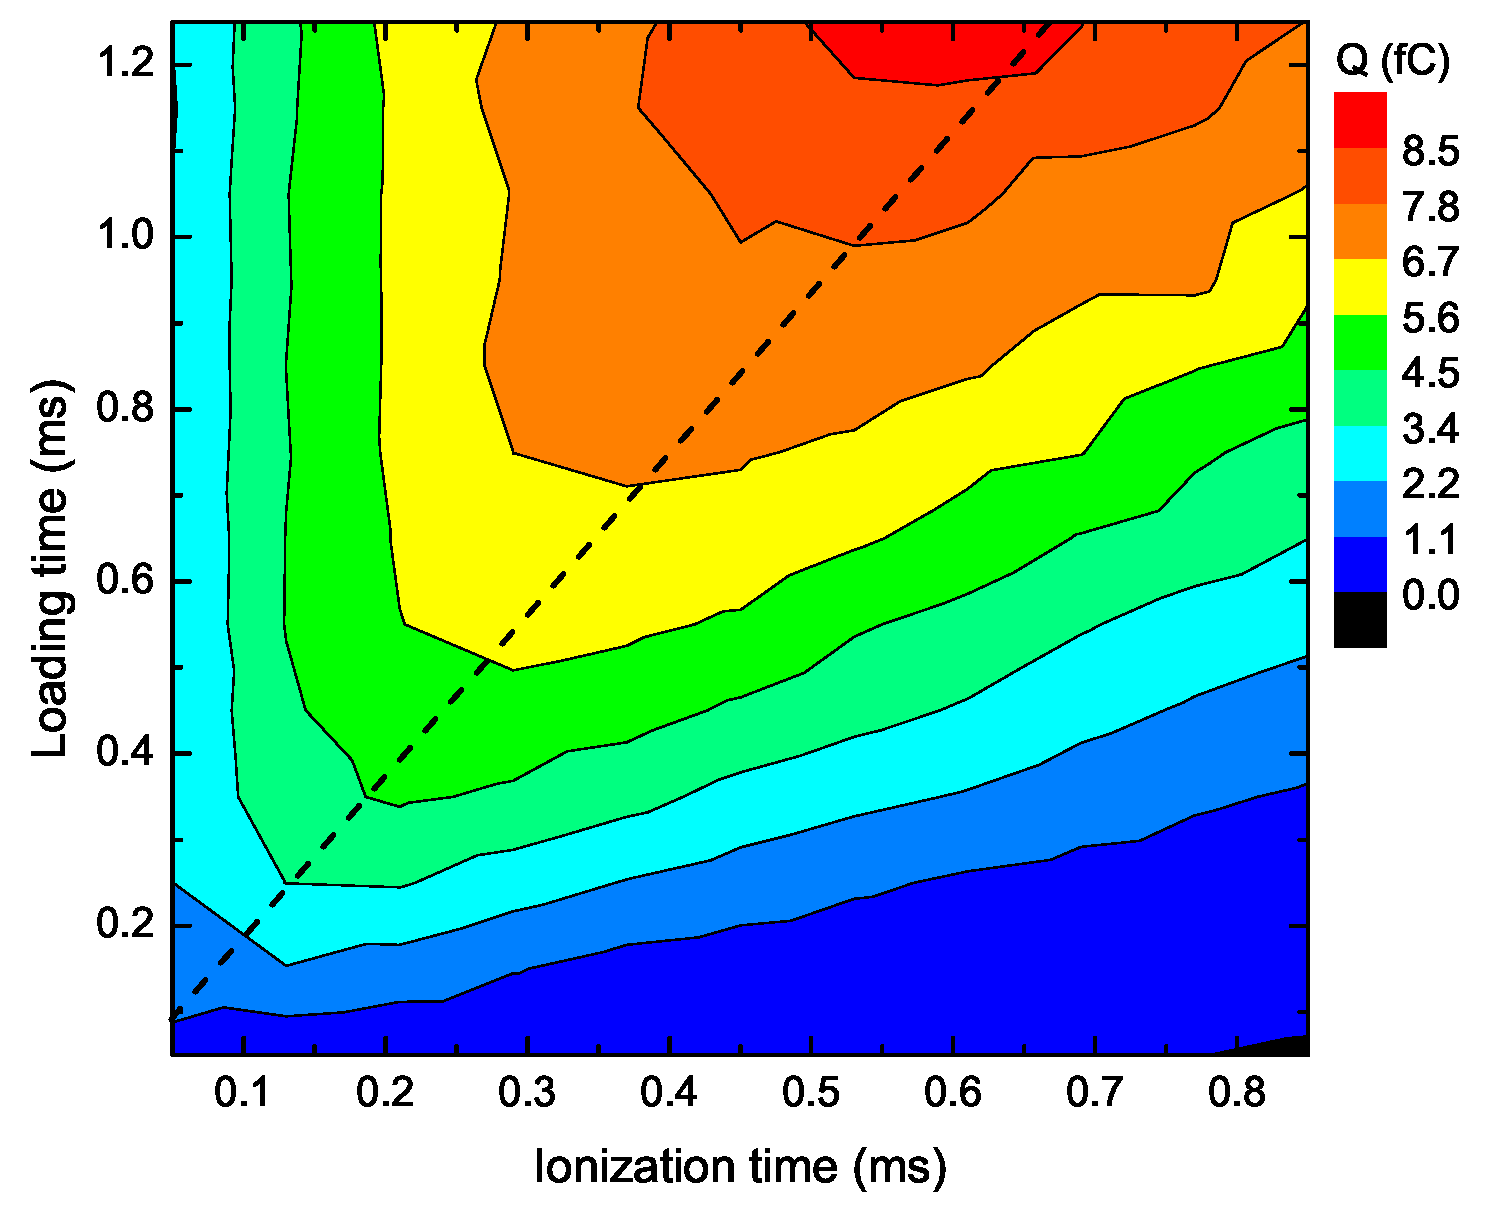
\includegraphics[width=0.6\linewidth]{pics/currmea/2DPlotChargeS=12.eps}
    \caption{Contour plot of the charge per pulse for $s_0=12$. Loading for a longer time leads to a larger charge, while ionizing for a longer time is not always beneficial.}
    \label{fig:charge2Dplot}
\end{figure}
The maximum in this graph is 8.8 fC, which corresponds to $5.5 \times 10^4$ ions. In general, longer loading and ionization times increase the charge per pulse, but the graph shows that there is a limit. In general, at a given loading time, increasing the ionization time will reduce the charge since a too long ionization time eventually reduces the available time to load atoms in the trap. The slope $\rho$ can also be defined for charge plots in a similar way as discussed in section \ref{sec:model} for the average current. In this case, $\rho=1.9$ (dashed line in the plot). The ratio is slightly smaller than for the average current of figure \ref{s2}. This is to be expected since a longer ionization time will result in some extra charge, but the period $t_{cycle}$ will be longer, reducing the average current. But since the slope is very similar, optimization of the average current coincides with optimization of the charge per pulse.\\

\noindent {\bf Ionization power dependence.} The power of the ionization laser beam used in the experiments is so small that removal of atoms by ionization can be neglected when determining the number of atoms in the core region. A change in the laser power therefore should not change the temporal behavior of the current pulses but just the number of ionized atoms. Figure \ref{fig:diffP} shows two contour plots from an experiment where the ionization laser power has been decreased by a factor 3.8 with the use of a neutral density filter.
\begin{figure*}[tbh!]
	\subfloat[$P_i=46$ mW\label{p1}]{\includegraphics[width=0.48\linewidth]{pics/currmea/2DPlotBigVolume}}
	\hfill	
	\subfloat[$P_i=12$ mW\label{p2}]{\includegraphics[width=0.48\linewidth]{pics/currmea/2DPlotBigVolumeQuarterIonisPower.eps}}
	\caption{Contour plots of the average current for two different values of the ionization laser beam power. The optimal slope $\rho$ is shown as a dashed line in the figure. A black dot marks the maximum of the average current.\label{fig:diffP}}
\end{figure*}
Here, the size of the core region in the three dimensions is $(39 \times 63 \times 71)$ $\mu$m$^3$ resulting in a volume $V_c=2.8 \times 10^{-12}$ m$^3$. Also, $t_l$ is incremented in steps of 150~$\mu$s between 50~$\mu$s and 1250~$\mu$s and $t_i$ ranges between 50 and 500 $\mu$s in steps of 75 $\mu$s, in total the scan consists of 63 points. As predicted, the shape of the contour in the two figures is very similar and the average current decreased by a factor of 4.1, similar to the decrease in laser power.\\

\noindent {\bf Summary plots.} In this section, two summary plots for several measurements performed with a core volume $V_c=2 \times 10^{-13}$ m$^3$ are presented. In figure \ref{fig:slopes}, the slopes $\rho$ at which the optimum of the average current occurs, are plotted versus the saturation parameter of the excitation laser beam.
\begin{figure}[tbh!]
    \centering
        \includegraphics[width=0.65\linewidth]{pics/currmea/SlopesVsS.eps}
    \caption{Compilation of the slopes from all the experiments done with $V_c=2.8 \times 10^{-12}$ m$^3$. Qualitatively, a larger saturation parameter corresponds to a larger slope.}
    \label{fig:slopes}
\end{figure}
When more measurements are available for a specific $s_0$, they correspond to measurements done at different ionization power. The large uncertainty bars are related to the linear fit not matching the real behavior perfectly, as $\rho$ is not a constant in practice. For this reason the plot is qualitative. It does appear, however, that the slope increases with increasing saturation parameter in agreement with the prediction of section \ref{sec:typcurrent} shown in figure \ref{fig:smallVdiffs}. In general, for increasing saturation parameter, a larger increase in the peak current is expected compared to an increase in the final current. Hence, the gain in charge obtained by ionizing for a longer time is offset by a reduction in the number of atoms if the loading time is not adjusted, so that it is instead beneficial to reduce the ionization time. This then leads to a higher optimal slope $\rho$.

In figure \ref{fig:peakcurrent}, the peak current is plotted versus the saturation parameter. A higher saturation parameter of the excitation laser beam means a higher excited state fraction and therefore a higher initial peak current. Hence, the expected behavior of the peak current is to be proportional to the excited state fraction: $I_{peak} \propto f(s_0,\delta~\rightarrow~0)$, from equation (\ref{eq:fraction}).
\begin{figure}[tbh!]
    \centering
        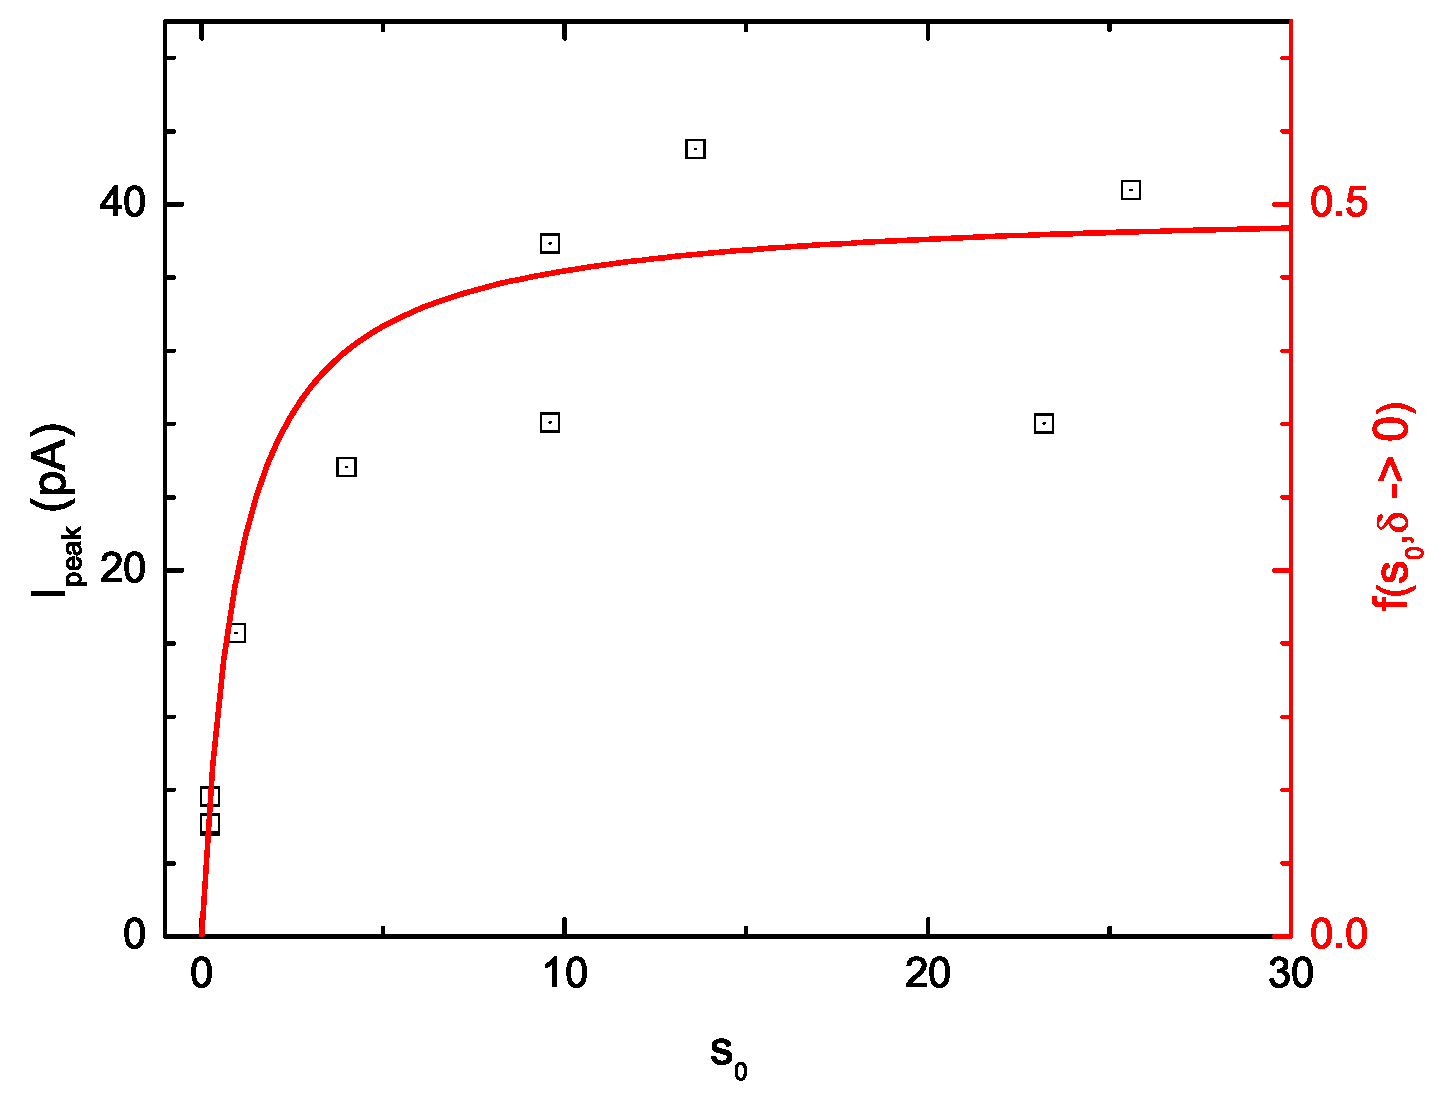
\includegraphics[width=0.7\linewidth]{pics/currmea/PeakCurrent.eps}
    \caption{Compilation of the peak current (on the left vertical axes) plotted versus the saturation parameter for several experiments with a core size $V_c=2.8 \times 10^{-12}$ m$^3$ and $P_i=46$~mW. The excited fraction $f(s_0,\delta \rightarrow 0)$ (on the right vertical axis) versus $s_0$ is plotted as a solid line.}
    \label{fig:peakcurrent}
\end{figure}
This relation is also plotted in the figure as a solid line. The shape of the curve indeed corresponds to the trend of the data points.

\section{Discussion and conclusion} \label{sec:conclusion}
To summarize, in this paper we described a semi-analytic model that allows one to calculate the current that can be extracted from an ultracold ion source under pulsed operation. An important feature of the model is that it takes into account the radiation pressure exerted by the excitation laser beam. This turns out to have an important influence on the magnitude and temporal behavior of the current because it pushes atoms through the ionization region. The model was used to predict the optimum settings of ionization and loading times to achieve maximum cycle-averaged current. Measurements of extracted currents show general agreement with the predictions in terms of temporal behavior, magnitude of the current, dependence on the position of the ionization volume, and loading and ionization times for which optimum current extraction is achieved. The key parameters of the model, i.e. the temperature of the atoms, the loading rate and lifetimes of the trap, were obtained from auxiliary experiments.  

For a core volume $V_c=2 \times 10^{-13}$ m$^3$, the maximum cycle-average current we obtained was $\overline{I}=(13 \pm 1)$~pA at $t_i=135$ $\mu$s and $t_l=250$ $\mu$s and $s_0=4$. This corresponds to a current density $J= \overline{I}/(2 \pi \sigma_x \sigma_y) = 4.9$ $10^{-3}$ A/m$^2$, where $\sigma_x=21~\mu$m and $\sigma_y = 20~\mu$m. If we assume that the transverse velocity spread of the ions is simply given by the temperature of the trapped atoms as found by Hanssen \emph{et al.} \cite{Hanssen_NL_08}, the transverse reduced brightness of the source is $B_r = Je/\pi k_b T_s= (8 \pm 1) \times 10^4$~A/m$^2$~sr~eV. This not far from the brightness of $3\times 10^5$~A/m$^2$~sr~eV we predicted as ultimately achievable in \cite{Geer_JoAP_07}, but it is obtained for an atom number density that is 40 times lower and a smaller ionization probability per atom than used in that estimate. This again illustrates the beneficial effect of the radiation pressure of the excitation laser beam, which effectively increases the atom number density in the core by a factor of $\sqrt{10}$ in each phase-space planes.

From the size of the ionization laser beam in the $z$-direction $\sigma_{i,z}=31$ $\mu$m and $V_a=800$ V, we calculate an \emph{rms} energy spread of the ion beam $\sigma_U=e \sigma_{i,z} E_0= 0.9$~eV, well below that of the LMIS, for an acceleration field $E_0=V_a/d_{eff}=29$ kV/m with $d_{eff}=27$~mm the effective length of the accelerator \cite{Taban_PRSAB_08}.

The brightness we estimate above is only an upper limit since the transverse velocity spread of the ion beam was not measured. At least two effects could lead to a higher temperature of the ions: heating of the atoms due scattering of the excitation beam, and heating of the ions due to Coulombic interactions \cite{Geer_JoAP_07,Steele_JAP_11}. First, acceleration of the atoms by the excitation beam for $t_i=135$ $\mu$s results in a velocity $v_z=4.61$~m/s and requires every atom to scatter $b\approx$~773 photons. This would lead to a transverse velocity spread equivalent to a temperature of $\sigma_T=(2b/3)T_r=191~\mu$K, where $T_r=0.37~\mu$K is the recoil temperature for Rb-85 \cite{Metcalf_Book_99}. This is comparable to the measured equilibrium temperature of the trapped atoms and should therefore have only a small effect on the source brightness.

Van der Geer \emph{et al} \cite{Geer_JoAP_07} and Steele \emph{et al.} \cite{Steele_JAP_11} have studied heating of ions extracted from a UCIS/MOTIS. For the current density we report here, these calculations indicate that Coulombic effects could have a significant influence for an acceleration field of 29~kV/m. We have therefore simulated extraction of the ions with the {\sc GPT} particle tracking code \cite{gpt} under conditions similar to the experiment. Here we assume a continuous atomic beam characterized by a Gaussian transverse density profile with 20~$\mu$m \textit{rms}-radius, traveling at 5~m/s and subject to an ionization rate with spatial variation according to a Gaussian with 31~$\mu$m \emph{rms} width. The 50\% reduced brightness \cite{Geer_JoAP_07} of the ion beam is calculated at a distance of 0.1~m behind the ionization region. The resulting reduced brightness of the ion beam is shown as a function of extracted current in figure~\ref{fig:GPTresult}, which shows that stochastic heating already decreases brightness starting at currents as low as 1~pA (solid curve in black). Since in the experiment peak currents of 50~pA are obtained, stochastic heating will be a dominating influence. To reduce the effect, the peak current should be reduced by operating the source in a continuous mode, and the magnitude of the accelerating field increased. To preserve the 1~eV energy spread, the ionization laser beam could be more narrowly focused. To exploit at best the pushing effect, the ionization laser beam can be moved to immediately behind the MOT in the positive $z$-direction (see figure~\ref{fig:setup}). The solid line in red in figure~\ref{fig:GPTresult}, show the case where an higher extraction voltage, $V_a=4$~kV, is used, leading to a higher energy spread $\sigma_U = 4.5$~eV. The energy spread is similar to the one of the LMIS and in under those circumstances the disorder induced heating is ignorable up to 10 pA extracted current.

\begin{figure}[tbh!]
    \centering
        \includegraphics[width=0.7\linewidth]{pics/currmea/GPTresult.eps}
    \caption{Simulated ion beam brightness as function of extracted current for conditions similar to the experiment. Dashed curves: Coulombic interactions excluded; solid curve: included (for two different energy spread values).}
    \label{fig:GPTresult}
\end{figure}
 
One conclusion we draw from the model is that the currently available ionization power of $P_i=46$~mW is insufficient to ionize all the atoms that pass through the ionization volume. Therefore it is possible to extract more current from the source by using a more intense ionization laser beam. To calculate this current, an extension of the model discussed in section \ref{sec:model} is required since the assumption above equation~\ref{eq:current} is no longer valid for a large $P_i$. In this extension of the model, the number of atoms will be corrected for the fraction of the atoms that have been ionized, $C_i$. In order to keep the calculation simple, this fraction is calculated as though the atoms move at a constant velocity in the core volume, resulting in
\begin{equation}
	C_i(t,z) = \exp\left(-r_i \cdot f(s_0,\delta(v_z)) \cdot \min\left(\frac{z+ \sigma_i \sqrt{\pi/2}}{v_z},t\right)\right).
  \label{eq:aveN2}
\end{equation}
The time spent in the core is limited to at most the time that the ionization laser beam is on. We can include depletion of the number of atoms by inserting the factor $C_i(t,z)$ in the integral in both equations (\ref{eq:Ncorecyl_unsolved}) and (\ref{eq:diffin2}). Figure \ref{fig:highpower} plots the calculated temporal dependence of the current for $P_i=$ 0.05, 0.5 and 5 W at $s_0=5$. 
\begin{figure}[tbh!]
    \centering
        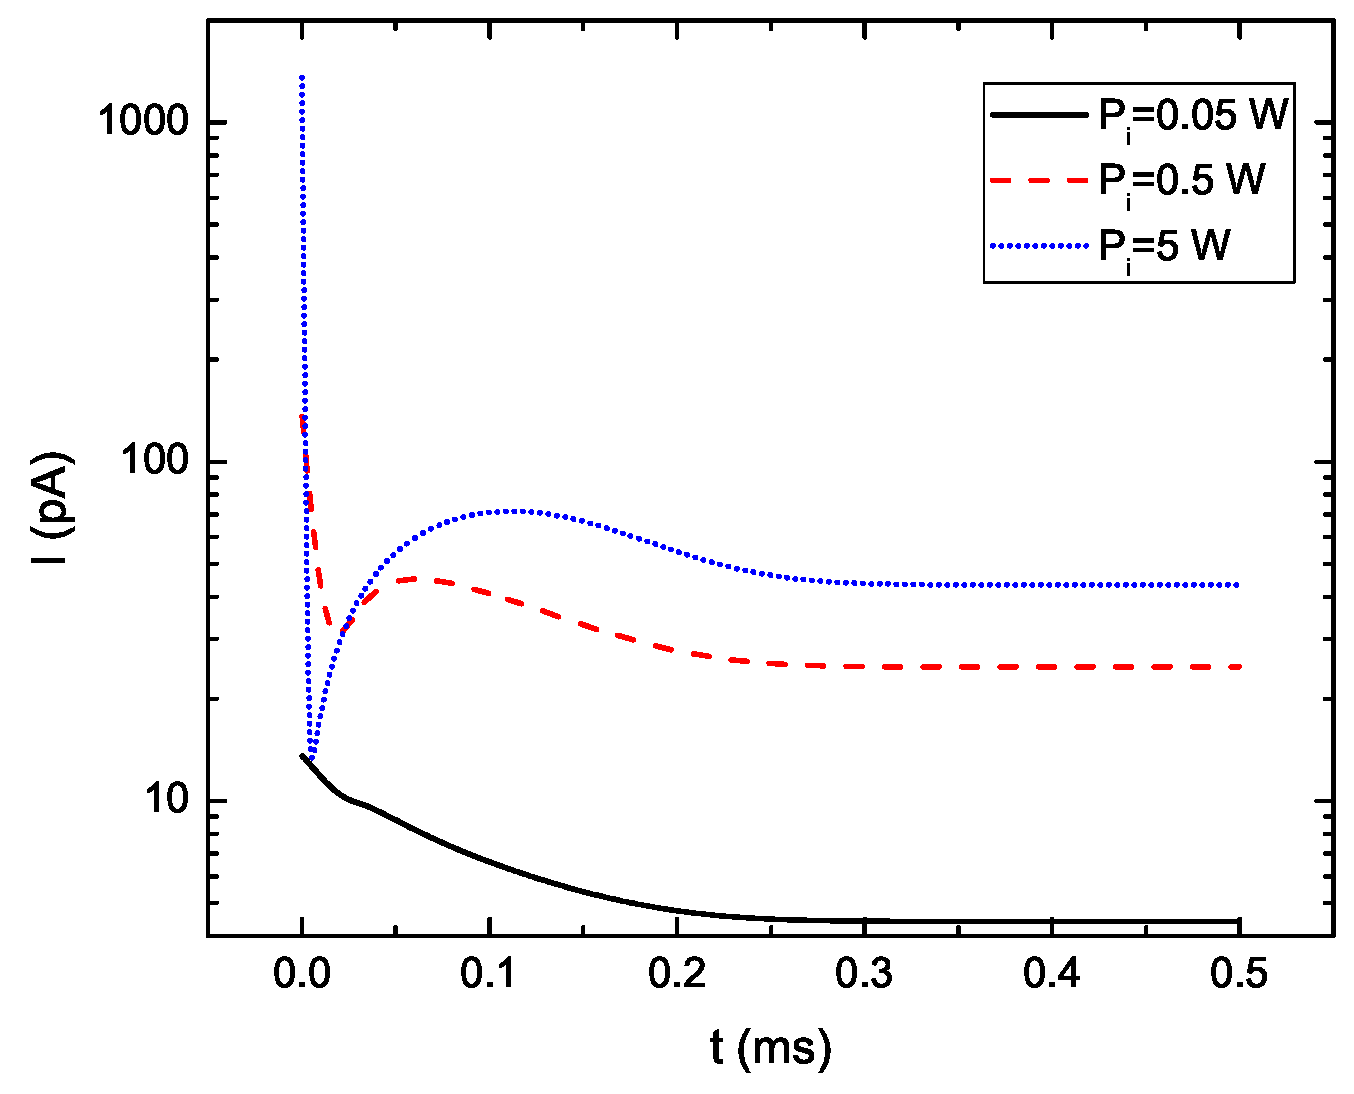
\includegraphics[width=0.7\linewidth]{pics/currmea/ModelHighIonisPower}
    \caption{A plot of the behavior of the modeled current in logarithmic scale over time for three different values of the ionization laser beam power with a saturation parameter $s_0=5$ of the excitation laser beam.}
    \label{fig:highpower}
\end{figure}
At large ionization power, the core region is quickly depleted so that the initial current is very large but decays in a very short time. After a while the current increases again due to the contribution of atoms pushed into the core region until it finally decreases to a steady level. For  large laser power, the temporal behavior of the current therefore does not resemble an exponential decay anymore. After optimizing loading and ionization times, we find that a maximum average current of $\overline{I} \approx 90$~pA should be possible at large power, $\approx$~7 times larger than for the current $P_i=0.05$ W. Even larger currents should be possible if the ionization volume is enlarged. However, at his point we run into another limitation of the model, which implicitly assumes that the extracted current represents only a small fraction of the loading rate of the trap, which corresponds to 190~pA. If this condition is violated, the atom number density in the trap (equation~\ref{eq:aveN}) is reduced by a substantial loss of atoms due to ionization, leading to lower than predicted currents. In practice this limitation could be overcome by increasing the rubidium vapor pressure, thereby increasing the loading rate. 


%\section{ACKNOWLEDGMENTS}
%The authors thank J. van de Ven, A. Kemper, W. Kemper, L. van Moll, E. Rietman, I. Koole and H. van Doorn for technical support. This research is supported by the Dutch Technology Foundation STW, applied science division of the ``Nederlandse Organisatie voor Wetenschappelijk Onderzoek (NWO)'' and the Technology Program of the Ministry of Economic Affairs.\\

\clearpage

\begin{subappendices}

\section{Extension to the DC source (UCIS$^+$)} \label{sec:extra}

Here we investigate operation of the source in DC mode as illustrated in figure~\ref{fig:source_CW}, in order to extract even higher beam currents.
\begin{figure}[tbh!]
    \centering
        \includegraphics[width=0.55\linewidth]{pics/currmea/source_CW}
    \caption{Schematic representation of the UCIS$^+$, not to scale. Differently than in figure \ref{fig:source}, the ionization lase beam is translated by $\delta z$ to better exploit the pushing effect of the excitation laser beam. An aperture is added to the setup.}
    \label{fig:source_CW}
\end{figure}
Differently than in figure \ref{fig:source}, the ionization lase beam is positioned at a positive distance $\delta z$ from the center of the MOT, to better exploit the pushing effect of the excitation laser beam. The power of the ionization laser beam is set at 5 W and the source is then renamed UCIS$^+$.

\begin{figure}[tbh!]
    \centering
        \includegraphics[width=0.6\linewidth]{pics/currmea/newsource08}
    \caption{The current $I_{DC}$ plotted versus $\sigma_i$ and $s_0$.}
    \label{fig:newsource}
\end{figure}

The approach is different from the one described in section \ref{sec:model}. The velocity $v_z$ of a particle being pushed by the excitation laser after a time $t$ is given by equation (\ref{eq:velocity}). The distance traveled by the particle is calculated from
\begin{equation}
	d(v_z) = \int_0^{v_z} \frac {v'_z} {a} d v'_z = \frac{m v_z^2}{\Gamma \hbar} \left( \frac{1}{k} + \frac{1}{k s_0} + \frac{2 k v_z^2}{\Gamma^2 s_0} \right),
  \label{eq:distance2}
\end{equation}
where the acceleration $a=F/m$ and the force $F$ are defined in equation (\ref{eq:force}). The current distribution is
\begin{equation}
	\frac{\partial I}{\partial v_z} = \frac{\partial I}{\partial d} \frac{\partial d}{\partial v_z} = K e^{\left( -(d(v_z)-\Delta z)^2 / {2 \sigma_M^2} \right)} e^{-t/\tau_d} \frac{v_z}{a},
  \label{eq:Idv}
\end{equation}
with $K=e \pi \sigma_e n_c \langle v \rangle  / \sqrt2$ including all constants and $\partial d/\partial v_z = v_z/a$ is calculated by derivation of equation \ref{eq:distance2} with respect to the velocity. The quantities $\langle v \rangle=0.3$ m/s, $n_c=2.5 \times 10^{16}$~m$^{-3}$ and $\delta z=\sigma_M =0.8$ mm are used for the calculations. The DC current extracted from the UCIS$^+$ $I_{DC}$ is then given by
\begin{equation}
	I_{DC} = \int_0^{v_z(t_{\infty})}{\frac{\partial I}{\partial v_z}} \left( 1 - p_s \right) d v,
  \label{eq:CWcurrent}
\end{equation}
where $p_s$ is the probability for a particle to ``survive'' the ionization process and is given by
\begin{equation}
	p_s=e^{-f r_i \sqrt{2 \pi} \sigma_i/v_z}.
  \label{eq:prob}
\end{equation}
The ionization rate is defined as in equation (\ref{eq:r_ion}) and the excited state fraction is $f=0.5$, since the trapping laser beams are always turned on.

Figure \ref{fig:newsource} show the current $I_{DC}$ plotted versus the excitation laser beam radius $\sigma_e$ and the saturation parameter of the excitation laser beam $s_0$. %, for $\Delta z=0,~\sigma_m,~2 \sigma_M$.
%\begin{figure*}[tbh!]
%	\subfloat[$\Delta z=0$ mm\label{cw1}]{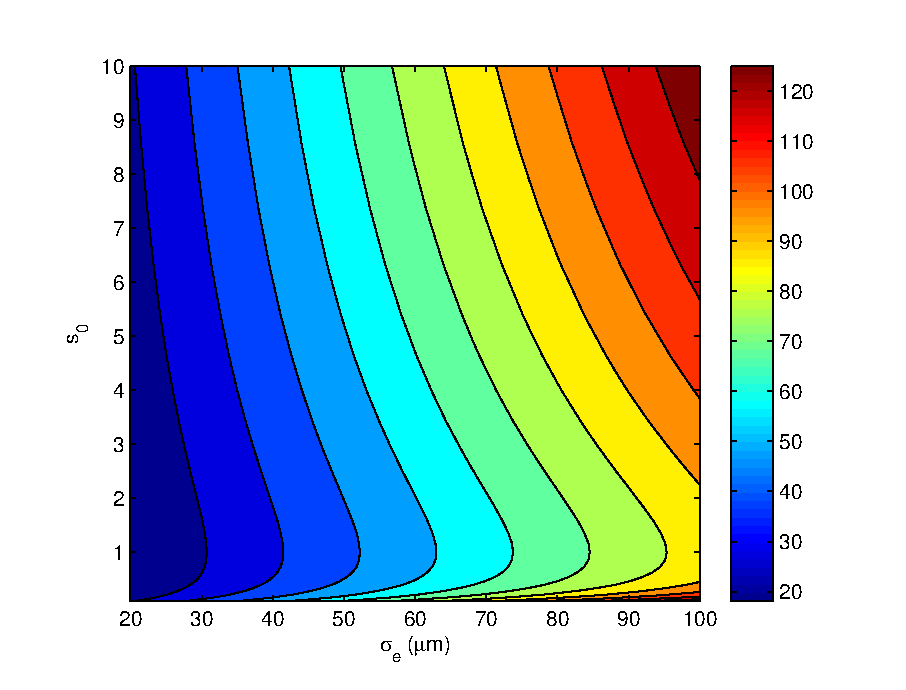
\includegraphics[width=0.48\linewidth]{pics/newsource0}}
%	\hfill	
%	\subfloat[$\Delta z=\sigma_M$\label{cw2}]{\includegraphics[width=0.48\linewidth]{pics/newsource08}}
%	\hfill
%	\centering	
%	\subfloat[$\Delta z=2 \sigma_M$\label{cw3}]{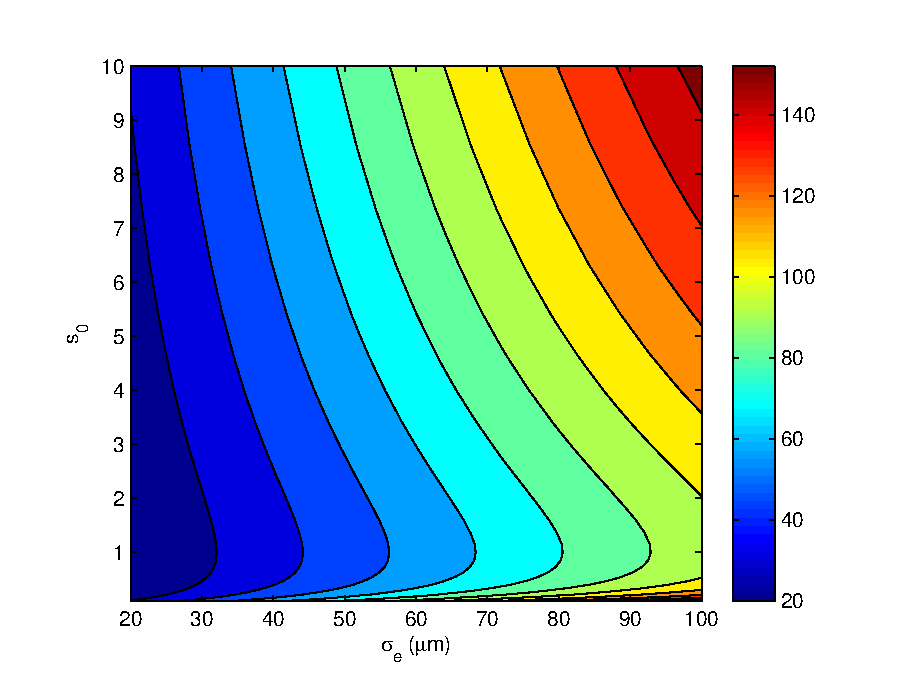
\includegraphics[width=0.48\linewidth]{pics/newsource16}}
%	\caption{The current $I_{DC}$ plotted versus $\sigma_i$ and $s_0$, for three values of $\Delta z$ (expressed in unit of $\sigma_M=0.8$ mm).\label{fig:newsource}}
%\end{figure*}
%From the results, it can be seen that the highest current are obtained at $\delta z = \sigma_M$. For a larger $\delta_z$, the diffusion out of the atoms outside of the cylinder becomes more important. Currents in the order of 100 pA can be extracted from the UCIS$^+$. This is achieved for instance using $s_0=1$ and $\sigma_e=100~\mu$m, which is still much smaller than $\sigma_M=0.8$ mm.\\
From the results, it can be seen that the highest current in the order of 100 pA can be extracted from the UCIS$^+$. This is achieved for instance using $s_0=1$ and $\sigma_e=100~\mu$m, which is still much smaller than $\sigma_M=0.8$ mm.
Disorder induced heating will still probably reduce the brightness as shown in figure \ref{fig:GPTresult} under the same conditions, but no simulation with GPT has been performed.

\end{subappendices}

\clearpage

\bibliographystyle{unsrt}
%
\begin{thebibliography}{10}

\bibitem{itrs}
http://www.itrs.net/.

\bibitem{Moore_E_65}
G.E. Moore.
\newblock {C}ramming more components onto integrated circuits.
\newblock {\em Electronics}, 38/8, 1965.

\bibitem{Hagen_J_08}
C.~W. Hagen, E.~Fokkema, and P.~Kruit.
\newblock {B}rightness measurements of a gallium liquid metal ion source.
\newblock {\em J Vac Sci Technol B}, 26(6):2091--2096, 2008.

\bibitem{Bell_JVSTB_88}
A.E. Bell, K.~Rao, G.A. Schwind, and L.W. Swanson.
\newblock {\em J. Vac. Sci. Technol. B}, 6:927--931, 1988.

\bibitem{Volkert2007}
C.~A. Volkert and A.~M. Minor.
\newblock Focused ion beam microscopy and micromachining.
\newblock {\em MRS Bulletin}, 32:389--399, 2007.

\bibitem{Kruit_NIaMiPRSAASDaAE_95}
P.~Kruit, L.~J. Vijgen, and Jiang Xinrong.
\newblock {C}oulomb interactions in microfocussed electron and ion beams.
\newblock {\em Nuclear Instruments and Methods in Physics Research Section A:
  Accelerators, Spectrometers, Detectors and Associated Equipment},
  363(1-2):220 -- 224, 1995.

\bibitem{Hanssen_PRA_06}
J.~L. Hanssen, J.~J. McClelland, E.~A. Dakin, and M.~Jacka.
\newblock {L}aser-cooled atoms as a focused ion-beam source.
\newblock {\em Phys. Rev. A: At. Mol. Opt. Phys.}, 74(6):063416, Dec 2006.

\bibitem{Geer_JoAP_07}
S.~B. van~der Geer, M.~P. Reijnders, M.~J. de~Loos, E.~J.~D. Vredenbregt,
  P.~H.~A. Mutsaers, and O.~J. Luiten.
\newblock {S}imulated performance of an ultracold ion source.
\newblock {\em J. Appl. Phys.}, 102(9):094312, 2007.

\bibitem{Metcalf_Book_99}
H.J. Metcalf and P.~van~der Straten.
\newblock {\em {L}aser {C}ooling and {T}rapping}.
\newblock Springer, 1999.

\bibitem{Steele_JVSTB_10}
A.~V. Steele, B.~Knuffman, J.~J. McClelland, and J.~Orloff.
\newblock {F}ocused chromium ion beam.
\newblock {\em J Vac Sci Technol B}, 28(6):C6F1--C6F5, 2010.

\bibitem{Reijnders_PRL_09}
M.~P. Reijnders, P.~A. van Kruisbergen, G.~Taban, S.~B. van~der Geer, P.~H.~A.
  Mutsaers, E.~J.~D. Vredenbregt, and O.~J. Luiten.
\newblock {L}ow-{E}nergy-{S}pread {I}on {B}unches from a {T}rapped {A}tomic
  {G}as.
\newblock {\em Phys. Rev. Lett.}, 102(3):034802, Jan 2009.

\bibitem{Hanssen_NL_08}
J.~L. Hanssen, S.~B. Hill, J.~Orloff, and J.~J. McClelland.
\newblock {M}agneto-{O}ptical-{T}rap-{B}ased, {H}igh {B}rightness {I}on
  {S}ource for {U}se as a {N}anoscale {P}robe.
\newblock {\em Nano Lett.}, 8(9):2844--2850, September 2008.

\bibitem{Debernardi_JAP_11}
N.~Debernardi, M.P. Reijnders, W.~J. Engelen, T.~T.~J. Clevis, P.~H.~A.
  Mutsaers, O.~J. Luiten, and E.~J.~D. Vredenbregt.
\newblock {M}easurement of the temperature of an ultracold ion source using
  time-dependent electric fields.
\newblock {\em J. Appl. Phys.}, 110:024501, 2011.

\bibitem{Steele_JAP_11}
A.~V. Steele, B.~Knuffman, and J.~J. McClelland.
\newblock {I}nter-ion coulomb interactions in a magneto-optical trap ion
  source.
\newblock {\em J. Appl. Phys.}, 109(10):104308, 2011.

\bibitem{Reijnders_PRL_10}
M.~P. Reijnders, N.~Debernardi, S.~B. van~der Geer, P.~H.~A. Mutsaers, E.~J.~D.
  Vredenbregt, and O.~J. Luiten.
\newblock {P}hase-{S}pace {M}anipulation of {U}ltracold {I}on {B}unches with
  {T}ime-{D}ependent {F}ields.
\newblock {\em Phys. Rev. Lett.}, 105(3):034802, Jul 2010.

\bibitem{Reijnders_JAP_11}
M.~P Reijnders, N.~Debernardi, S.B. van~der Geer, P.H.A. Mutsaers, E.J.D.
  Vredenbregt, and O.J. Luiten.
\newblock {T}ime-dependent manipulation of ultracold ion bunches.
\newblock {\em J. Appl. Phys.}, 109:033302, 2011.

\bibitem{Foot_Book_05}
C.~J. Foot.
\newblock {\em {A}tomic {P}hysics}.
\newblock Oxford University Press, 2005.

\bibitem{Taban_PRSAB_08}
G.~Taban, M.~P. Reijnders, S.~C. Bell, S.~B. van~der Geer, O.~J. Luiten, and
  E.~J.~D. Vredenbregt.
\newblock {D}esign and validation of an accelerator for an ultracold electron
  source.
\newblock {\em Phys. Rev. Spec. Top. Accel Beams}, 11(5):050102, 2008.

\bibitem{Monroe_PRL_90}
C.~Monroe, W.~Swann, H.~Robinson, and C.~Wieman.
\newblock {V}ery cold trapped atoms in a vapor cell.
\newblock {\em Phys. Rev. Lett.}, 65(13):1571--1574, Sep 1990.

\bibitem{Gabbanini_OC_97}
C.~Gabbanini, S.~Gozzini, and A.~Lucchesini.
\newblock {P}hotoionization cross section measurement in a {R}b vapor cell
  trap.
\newblock {\em Optics Communications}, 141(1-2):25 -- 28, 1997.

\bibitem{Weiss_JB_89}
D.S. Weiss, E.~Riis, Y.~Shevy, P.J. Ungar, and S.~Chu.
\newblock {O}ptical molasses and multilevel atoms: experiment.
\newblock {\em JOSA B}, 6:2072--2083, 1989.

\bibitem{gpt}
http://www.pulsar.nl/gpt.

\end{thebibliography}

%
%\end{document}
